\subsection{W+Jets MC Modelling Validation from CR1}
\label{sec:cr1}


The estimate of the uncertainty on this background is based on CR1, 
defined by applying the full signal selection, including the isolated track veto, but requiring 0 b-tags
(CSV medium working point as described in Sec.~\ref{sec:selection}). 
The sample is dominanted by \wjets\ and is thus used to validate the MC modelling of this background. 

In Table~\ref{tab:cr1mtsf} we show the amount that we need to scale the Wjets MC
by in order to have agreement between data and Monte Carlo in the $M_T$ peak 
region, defined as $50 < M_T < 80$ GeV, for the 
different signal regions.  (Recall, the signal regions have different
\met\ requirements).  These scale factors are not terribly 
important, but it is reassuring that they are not too different from
1. 


\begin{table}[!h]
\begin{center}
{\footnotesize
\begin{tabular}{l||c||c|c|c|c|c|c|c}
\hline
Sample              & CR1PRESEL & CR1A & CR1B & CR1C & CR1D & CR1E &
CR1F & CR1G\\
\hline
\hline
$\mu$ \mt-SF 	  & $0.92 \pm 0.02$ & $0.97 \pm 0.03$ & $0.90 \pm 0.04$ & $0.91 \pm 0.06$ & $0.93 \pm 0.09$ & $0.98 \pm 0.13$ & $0.94 \pm 0.18$ & $0.96 \pm 0.25$ \\
\hline
\hline
e \mt-SF 	  & $0.94 \pm 0.02$ & $0.90 \pm 0.04$ & $0.84 \pm 0.05$ & $0.80 \pm 0.07$ & $0.83 \pm 0.10$ & $0.77 \pm 0.13$ & $0.86 \pm 0.20$ & $0.87 \pm 0.29$ \\
\hline
\end{tabular}}
\caption{ \mt\ peak Data/MC scale factors applied to Wjets
  samples.   The MC is used for backgrounds from rare
  processes. CR1PRESEL refers to a sample with $\met>50$ GeV.
  The uncertainties are statistical only.
\label{tab:cr1mtsf}}
\end{center}
\end{table}

Next, in Fig~\ref{fig:cr1met},~\ref{fig:cr1mtrest},
and~\ref{fig:cr1mtrest2}, we show plots of \met\ and then $M_T$
for different \met\ requirements corresponding to those defining our signal regions.
It is clear that there are more events in the $M_T$ tail than
predicted
from MC. This implies that we need to rescale the MC Wjets
background
in the tail region.

\begin{table}[!h]
\begin{center}
{\footnotesize
\begin{tabular}{l||c||c|c|c|c|c|c|c}
\hline
Sample              & CR1PRESEL & CR1A & CR1B & CR1C & CR1D & CR1E &
CR1F & CR1G\\
\hline
\hline
$\mu$ MC 		  & $480 \pm 22$ & $173 \pm 5$ & $114 \pm 4$ & $40 \pm 2$ & $16 \pm 1$ & $8 \pm 1$ & $4 \pm 1$ & $2 \pm 1$ \\
$\mu$ Data 		  & $629$ & $238$ & $139$ & $45$ & $12$ & $8$ & $3$ & $2$ \\
\hline
$\mu$ Data/MC 	  & $1.31 \pm 0.08$ & $1.37 \pm 0.10$ & $1.22 \pm 0.11$ & $1.12 \pm 0.18$ & $0.75 \pm 0.23$ & $0.99 \pm 0.37$ & $0.75 \pm 0.45$ & $0.96 \pm 0.72$ \\
\hline
\hline
e MC 		  & $330 \pm 8$ & $118 \pm 4$ & $79 \pm 3$ & $29 \pm 2$ & $13 \pm 1$ & $5 \pm 1$ & $3 \pm 1$ & $2 \pm 0$ \\
e Data 		  & $473$ & $174$ & $100$ & $36$ & $16$ & $5$ & $5$ & $2$ \\
\hline
e Data/MC 	  & $1.43 \pm 0.07$ & $1.47 \pm 0.12$ & $1.27 \pm 0.14$ & $1.23 \pm 0.22$ & $1.26 \pm 0.34$ & $1.07 \pm 0.51$ & $1.80 \pm 0.91$ & $1.26 \pm 0.97$ \\
\hline
\hline
$\mu$+e MC 		  & $810 \pm 23$ & $291 \pm 7$ & $192 \pm 5$ & $69 \pm 3$ & $29 \pm 2$ & $13 \pm 1$ & $7 \pm 1$ & $4 \pm 1$ \\
$\mu$+e Data 		  & $1102$ & $412$ & $239$ & $81$ & $28$ & $13$ & $8$ & $4$ \\
\hline
$\mu$+e Data/MC 	  & $1.36 \pm 0.08$ & $1.42 \pm 0.13$ & $1.24 \pm 0.15$ & $1.17 \pm 0.23$ & $0.97 \pm 0.31$ & $1.02 \pm 0.51$ & $1.18 \pm 0.69$ & $1.09 \pm 0.96$ \\
\hline
\hline
\hline
$\mu$ W MC 		  & $300 \pm 23$ & $84 \pm 5$ & $52 \pm 4$ & $20 \pm 2$ & $9 \pm 2$ & $5 \pm 1$ & $3 \pm 1$ & $1 \pm 1$ \\
$\mu$ W Data 	  & $449 \pm 26$ & $149 \pm 16$ & $78 \pm 12$ & $25 \pm 7$ & $5 \pm 4$ & $5 \pm 3$ & $2 \pm 2$ & $1 \pm 1$ \\
\hline
$\mu$ W Data/MC 	  & $1.50 \pm 0.14$ & $1.77 \pm 0.21$ & $1.49 \pm 0.26$ & $1.25 \pm 0.38$ & $0.56 \pm 0.39$ & $0.98 \pm 0.62$ & $0.60 \pm 0.73$ & $0.94 \pm 1.14$ \\
\hline
\hline
e W MC 		  & $192 \pm 8$ & $55 \pm 4$ & $36 \pm 3$ & $14 \pm 2$ & $6 \pm 1$ & $3 \pm 1$ & $2 \pm 1$ & $1 \pm 0$ \\
e W Data 	  & $335 \pm 22$ & $111 \pm 13$ & $58 \pm 10$ & $20 \pm 6$ & $10 \pm 4$ & $3 \pm 2$ & $4 \pm 2$ & $1 \pm 1$ \\
\hline
e W Data/MC 	  & $1.74 \pm 0.14$ & $2.02 \pm 0.29$ & $1.58 \pm 0.32$ & $1.49 \pm 0.50$ & $1.50 \pm 0.70$ & $1.10 \pm 0.80$ & $2.27 \pm 1.55$ & $1.51 \pm 1.96$ \\
\hline
\hline
$\mu$+e W MC 		  & $493 \pm 24$ & $139 \pm 6$ & $89 \pm 5$ & $33 \pm 3$ & $16 \pm 2$ & $8 \pm 1$ & $4 \pm 1$ & $2 \pm 1$ \\
$\mu$+e W Data 	  & $785 \pm 59$ & $260 \pm 37$ & $135 \pm 28$ & $45 \pm 16$ & $15 \pm 9$ & $8 \pm 7$ & $6 \pm 5$ & $3 \pm 3$ \\
\hline
$\mu$+e W Data/MC 	  & $1.59 \pm 0.14$ & $1.87 \pm 0.28$ & $1.53 \pm 0.33$ & $1.35 \pm 0.50$ & $0.95 \pm 0.58$ & $1.03 \pm 0.83$ & $1.29 \pm 1.13$ & $1.16 \pm 1.65$ \\
\hline
\hline
\hline
$SFR_{wjet}$ 	  & $1.48 \pm 0.26$  & $1.64 \pm 0.38$  & $1.38 \pm 0.30$  & $1.26 \pm 0.39$  & $0.96 \pm 0.45$  & $1.02 \pm 0.67$  & $1.23 \pm 0.92$  & $1.12 \pm 1.31$  \\
\hline
\end{tabular}}
\caption{ Yields in \mt\ tail comparing the MC prediction (after
  applying SFs) to data. CR1PRESEL refers to a sample with $\met>50$
  GeV and $\mt>150$ GeV.  See text for details.
%   The uncertainties are statistical only. 
\label{tab:cr1yields}}
\end{center}
\end{table}


The rescaling is explored
in Table~\ref{tab:cr1yields},
Here we compare the data and MC yields in the $M_T$ signal regions
and in a looser control region.  Note that the 
MC is normalized in the $M_T$ peak region by rescaling 
the \wjets\ component according to Table~\ref{tab:cr1mtsf}.

We also derive data/MC scale factors.
These are derived in two different ways, separately for muons and
electrons and then combined, as follows;
\begin{itemize}
\item For the first three sets of scale factors, above the triple horizontal
  line, we calculate the scale factor as the amount by which we would
  need to rescale {\bf all} MC (\wjets\ , \ttbar\ , single top, rare) in
  order to have data-MC agreement in the $M_T$ tail.
\item For the next three set of scale factors, below the triple horizontal
line, we calculate the scale factor as the amount by which we would
need 
to scale \wjets\ keeping all other 
components fixed in order to have data-MC agreement in the tail.
\end{itemize}
\noindent  The true \wjets\ scale factor is somewhere in between these
two extremes.  We also note that there is no statistically significant
difference between the electron and muon samples.  We use these data
to extract a data/MC scale factor for \wjets\ which will be used to
rescale the \wjets\ MC tail.  This scale factor is listed in the last
line of the Table, and is called $SFR_{wjets}$.  It is calculated as
follows.
\begin{itemize}
\item Separately for each signal region
\item As the average of the two methods described above
\item Including the statistical uncertainty
\item Adding in quadrature to the uncertainty one-half of the
  deviation from 1.0
\end{itemize}

 




\begin{figure}[hbt]
  \begin{center}
        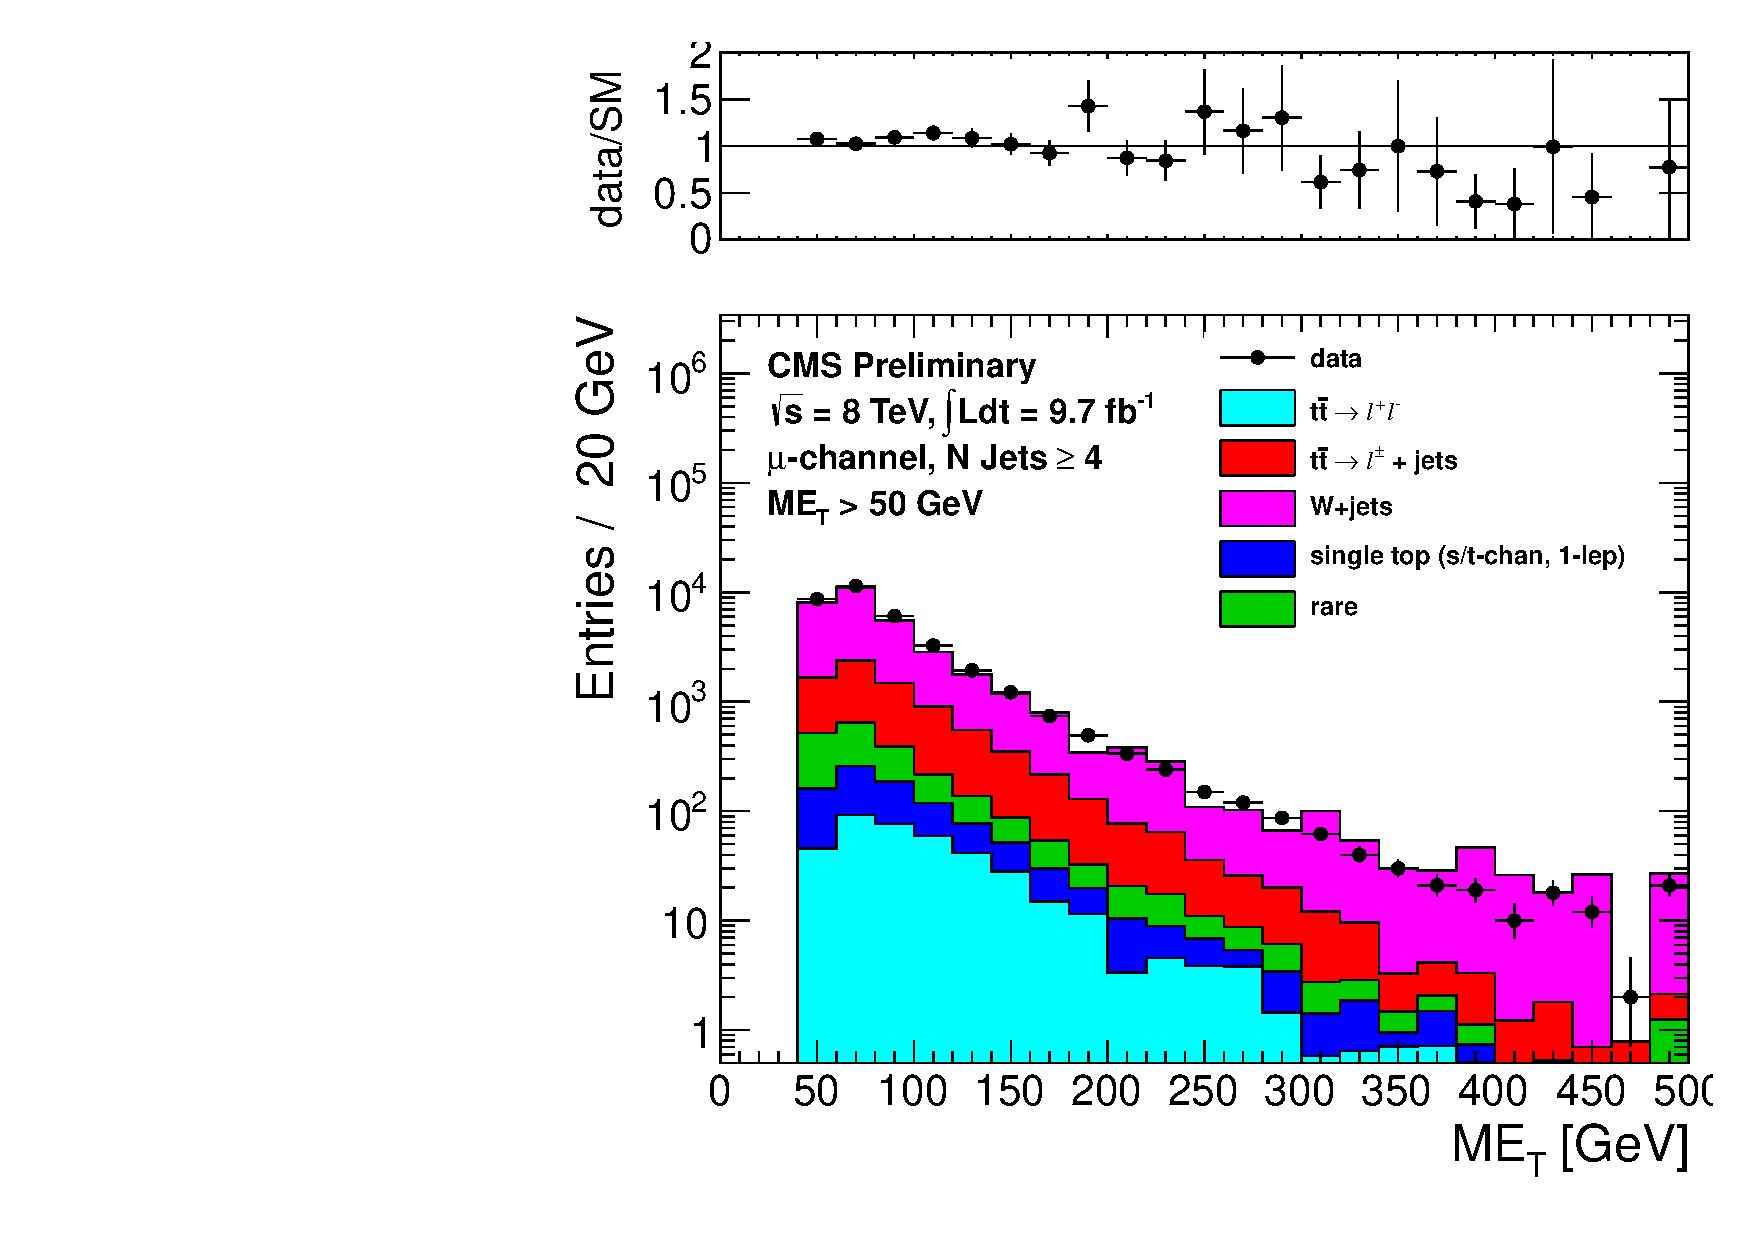
\includegraphics[width=0.5\linewidth]{plots/CR1plots/met_met50_leadmuo_nj4.pdf}%
        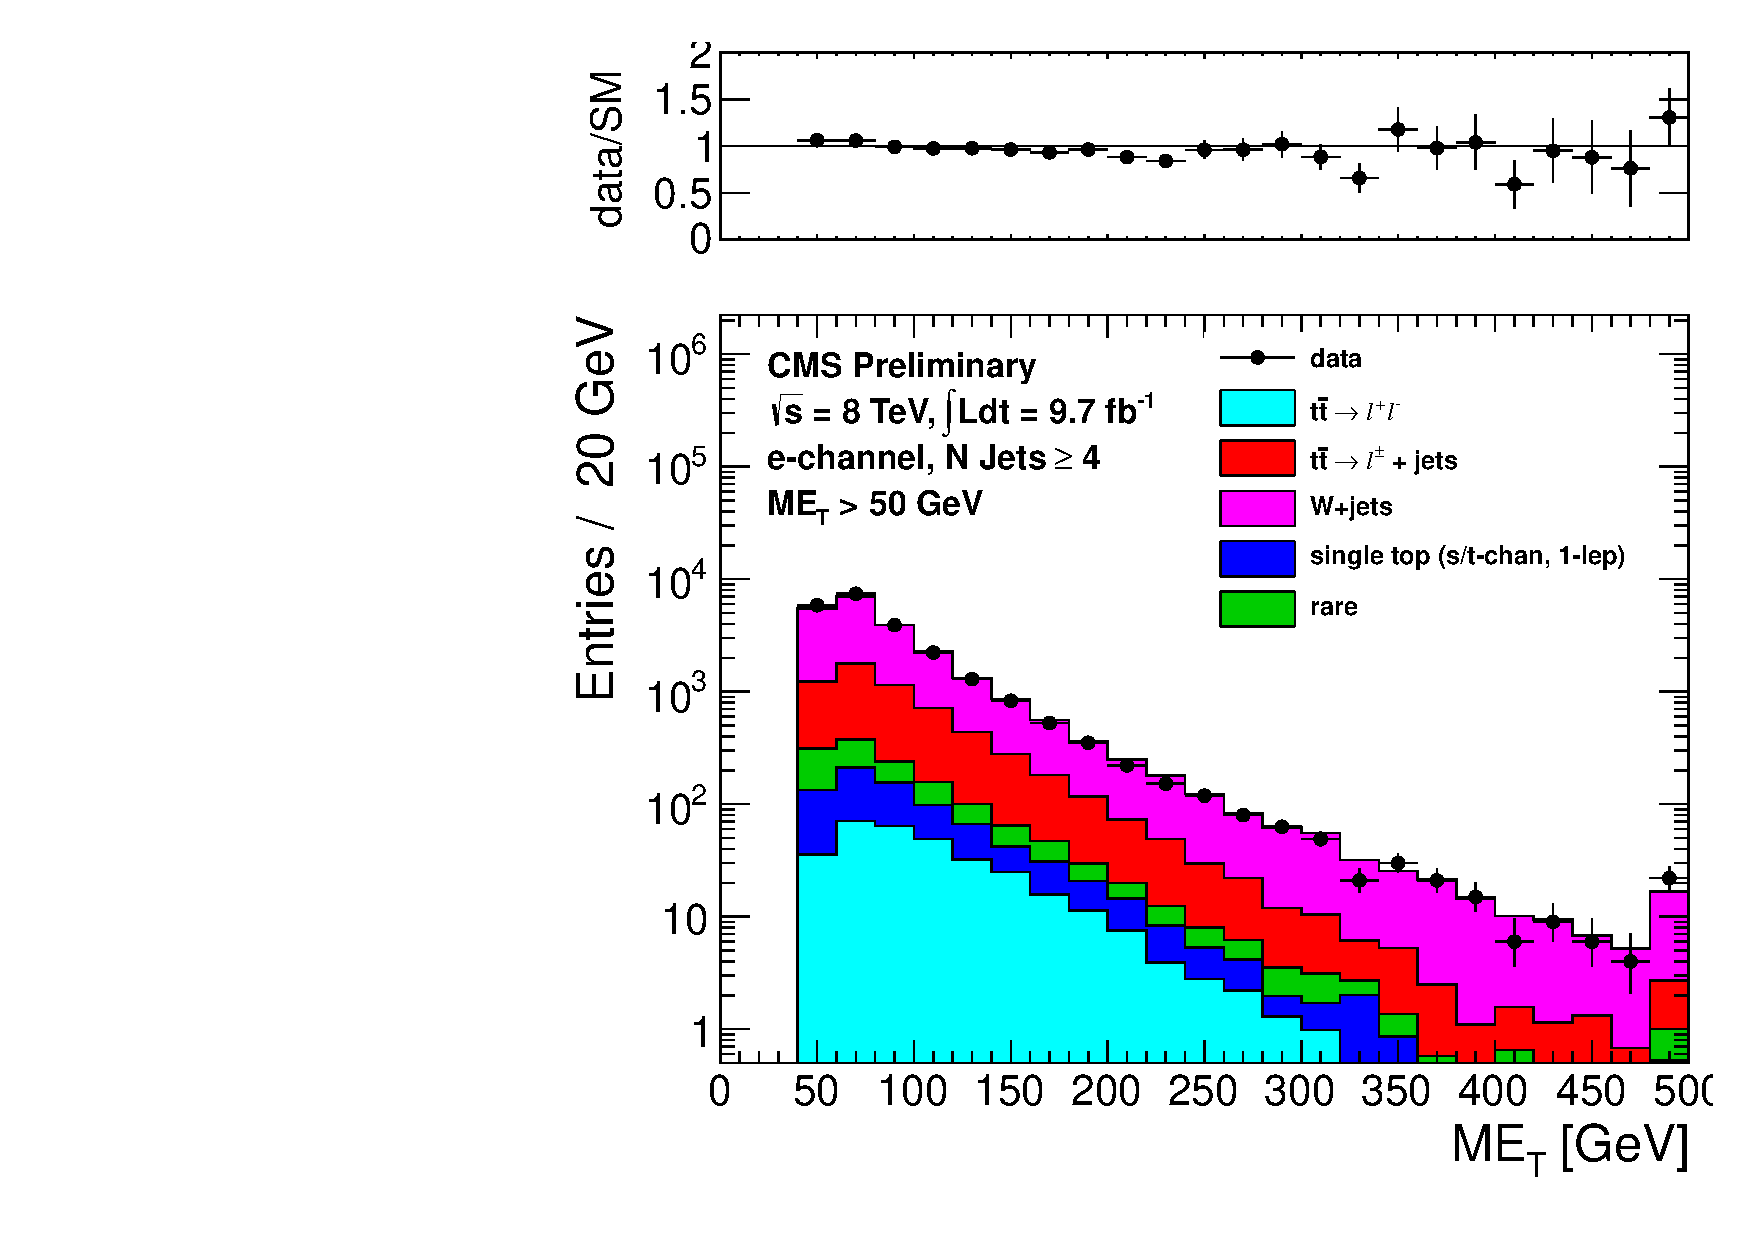
\includegraphics[width=0.5\linewidth]{plots/CR1plots/met_met50_leadele_nj4.pdf}
        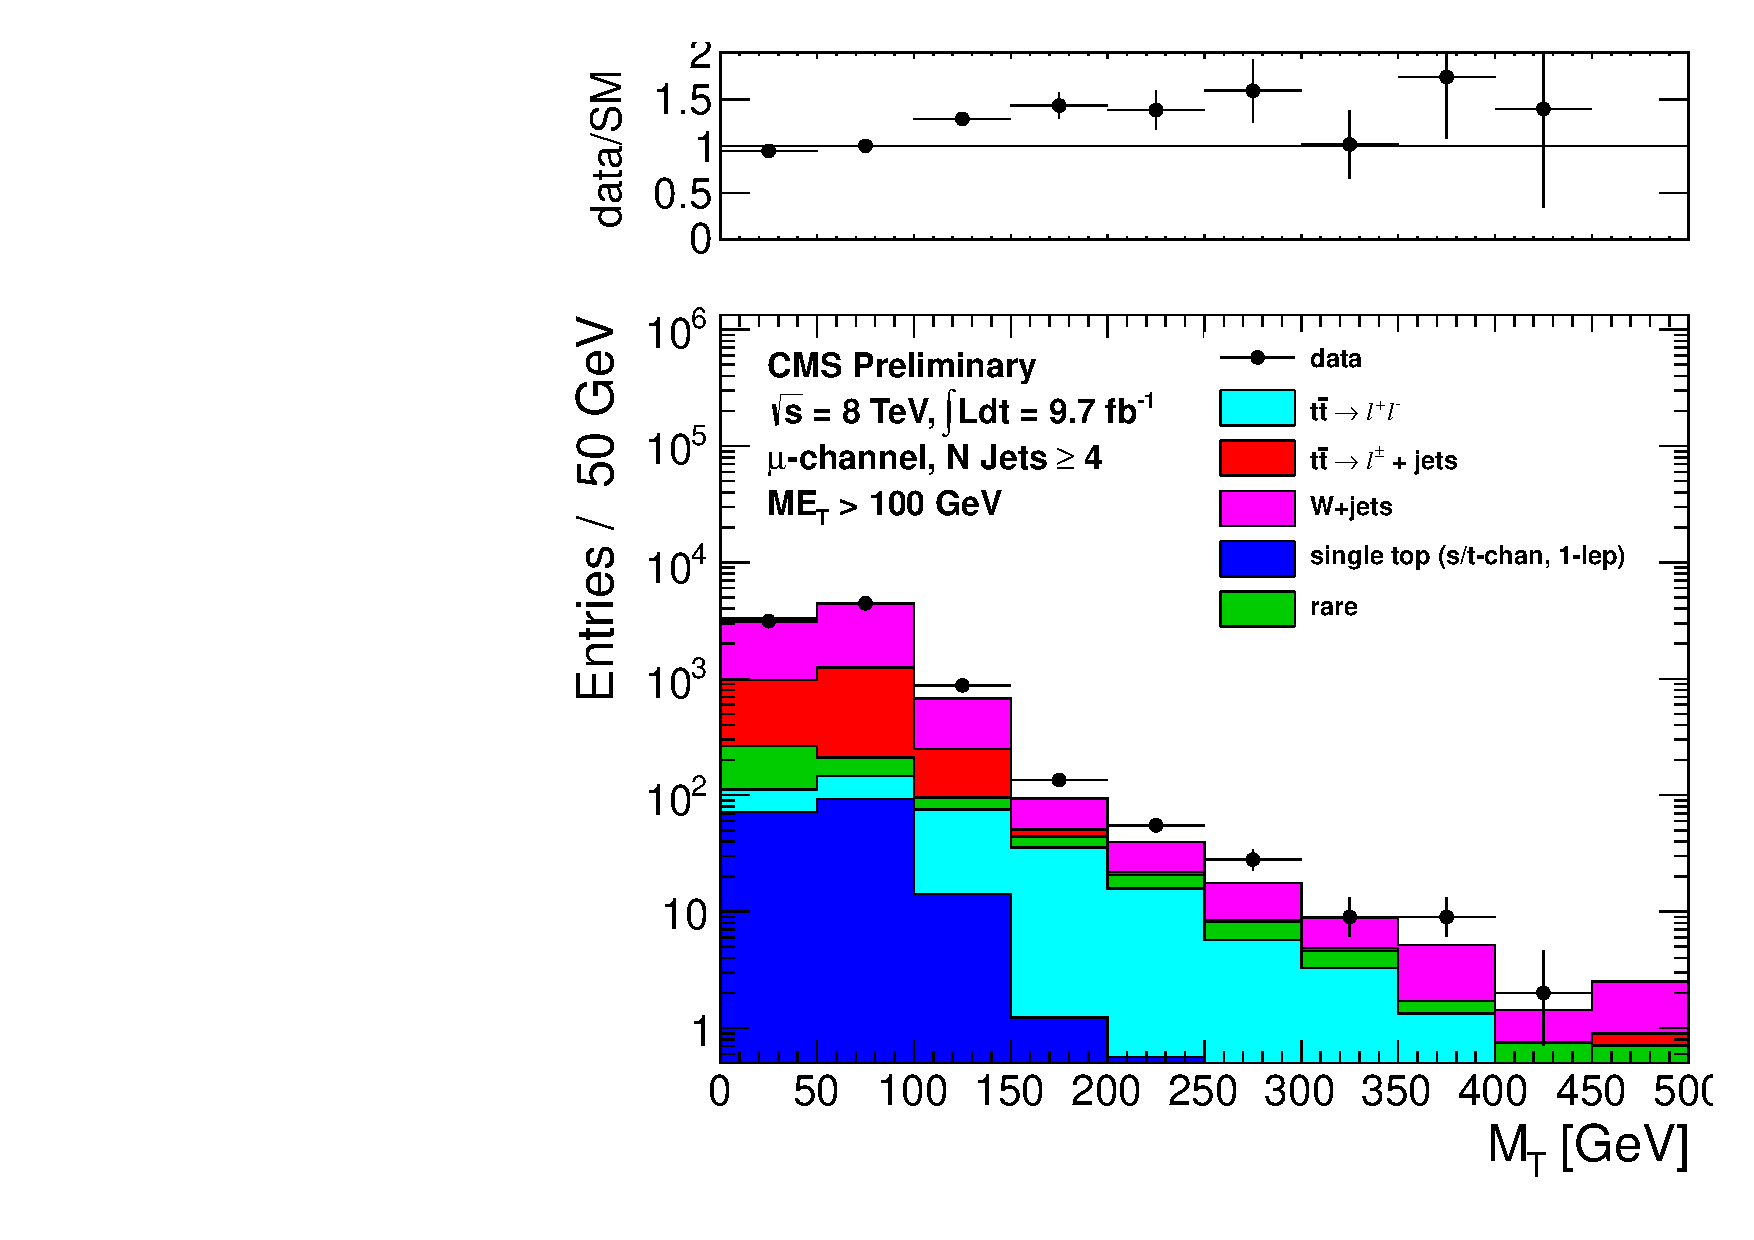
\includegraphics[width=0.5\linewidth]{plots/CR1plots/mt_met100_leadmuo_nj4.pdf}%
        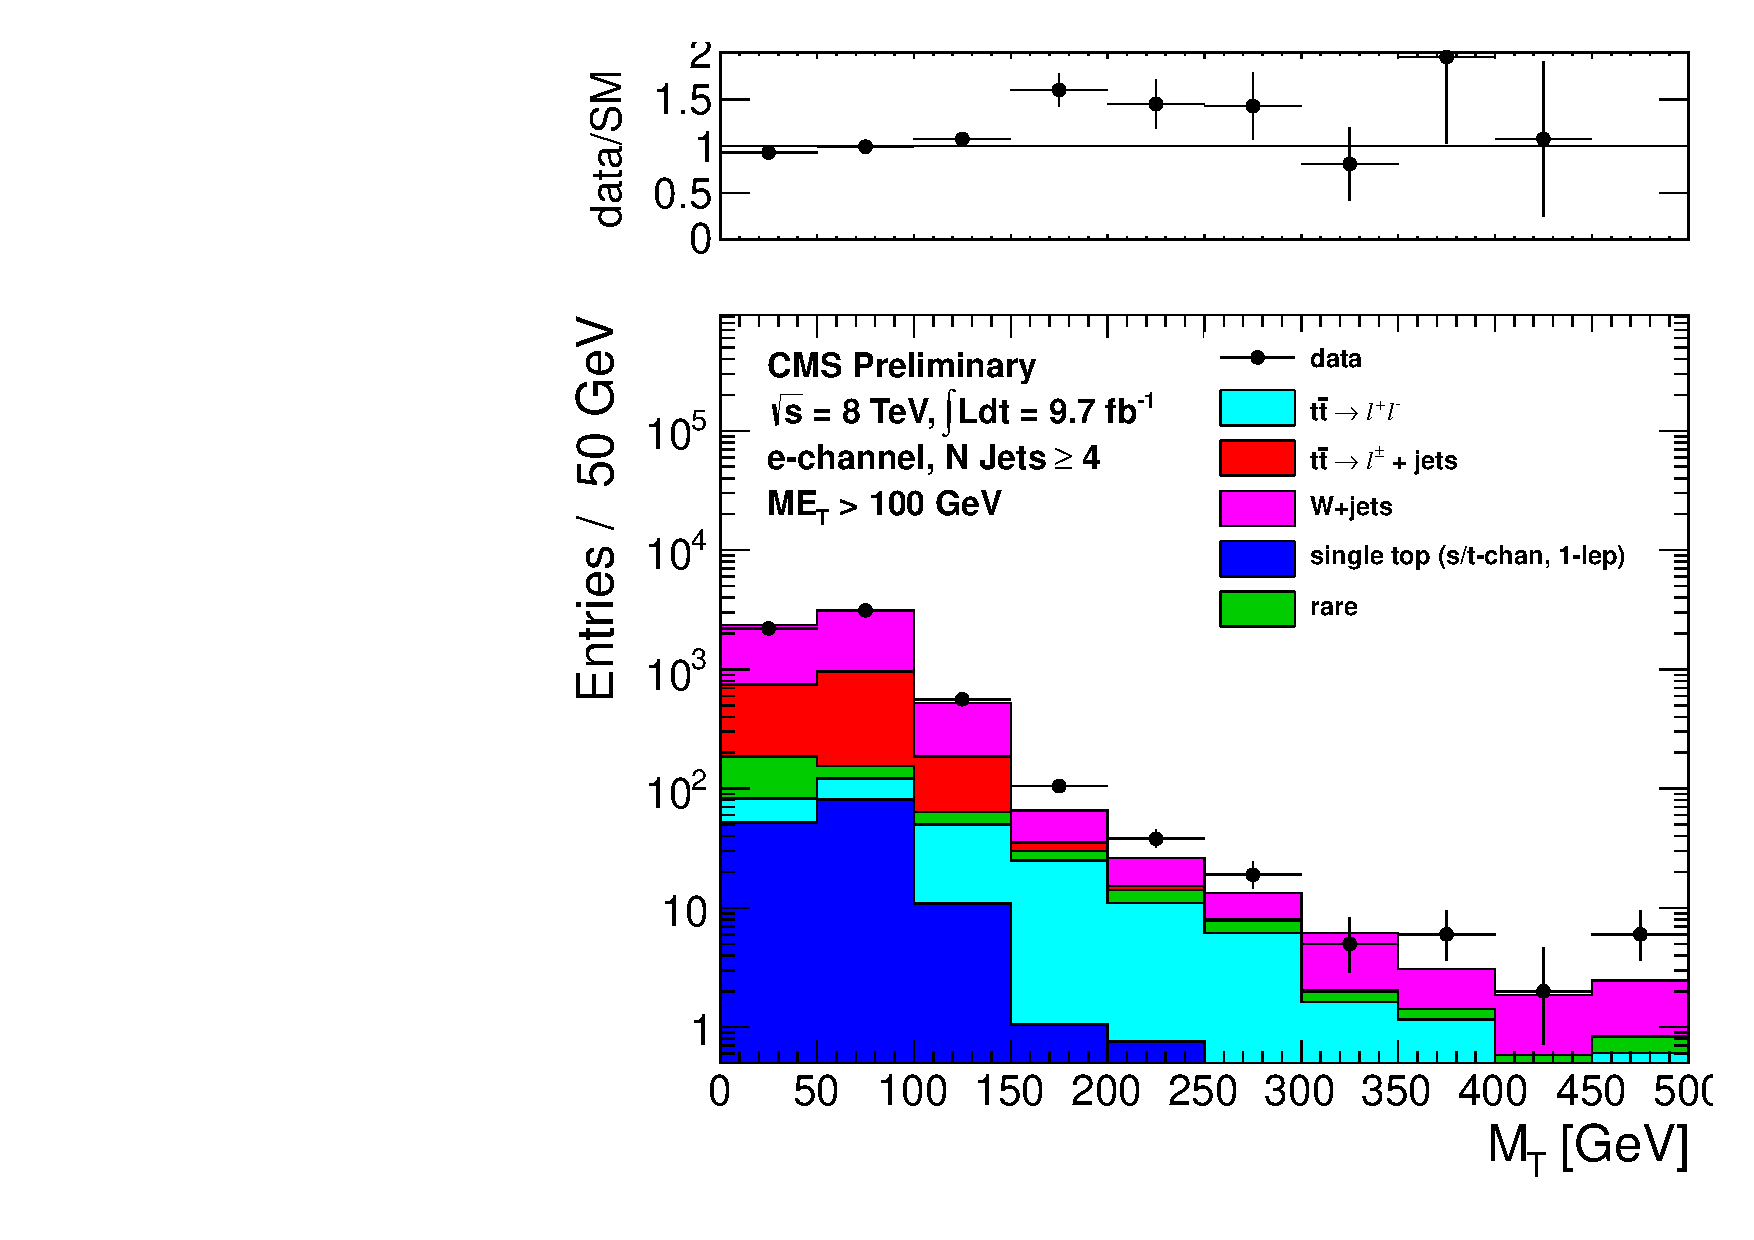
\includegraphics[width=0.5\linewidth]{plots/CR1plots/mt_met100_leadele_nj4.pdf}
    \caption{
      Comparison of the \met\ (top) and \mt\ for $\met>100$ (bottom) distributions in data vs. MC for events
      with a leading muon (left) and leading electron (right)
      satisfying the requirements of CR1. 
\label{fig:cr1met} 
}  
      \end{center}
\end{figure}


\begin{figure}[hbt]
  \begin{center}
        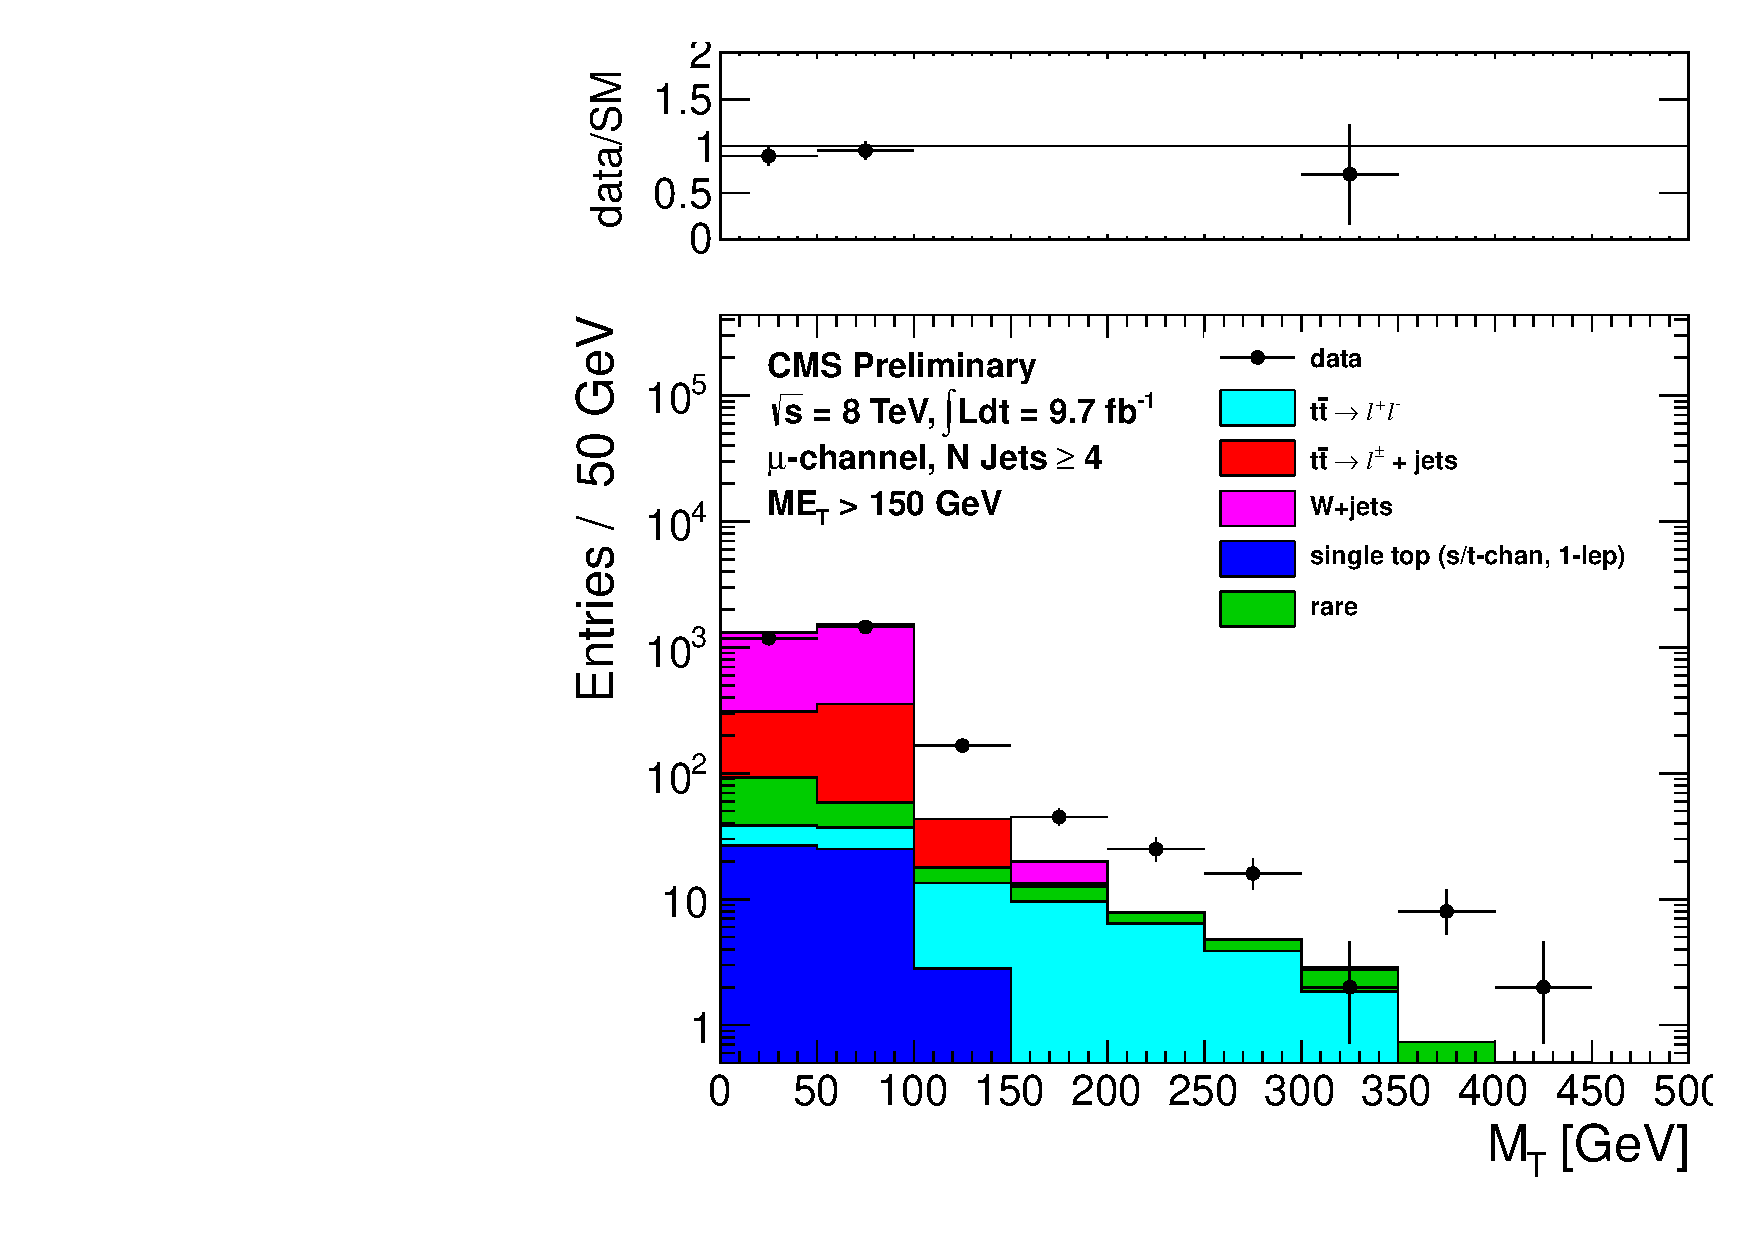
\includegraphics[width=0.5\linewidth]{plots/CR1plots/mt_met150_leadmuo_nj4.pdf}%
        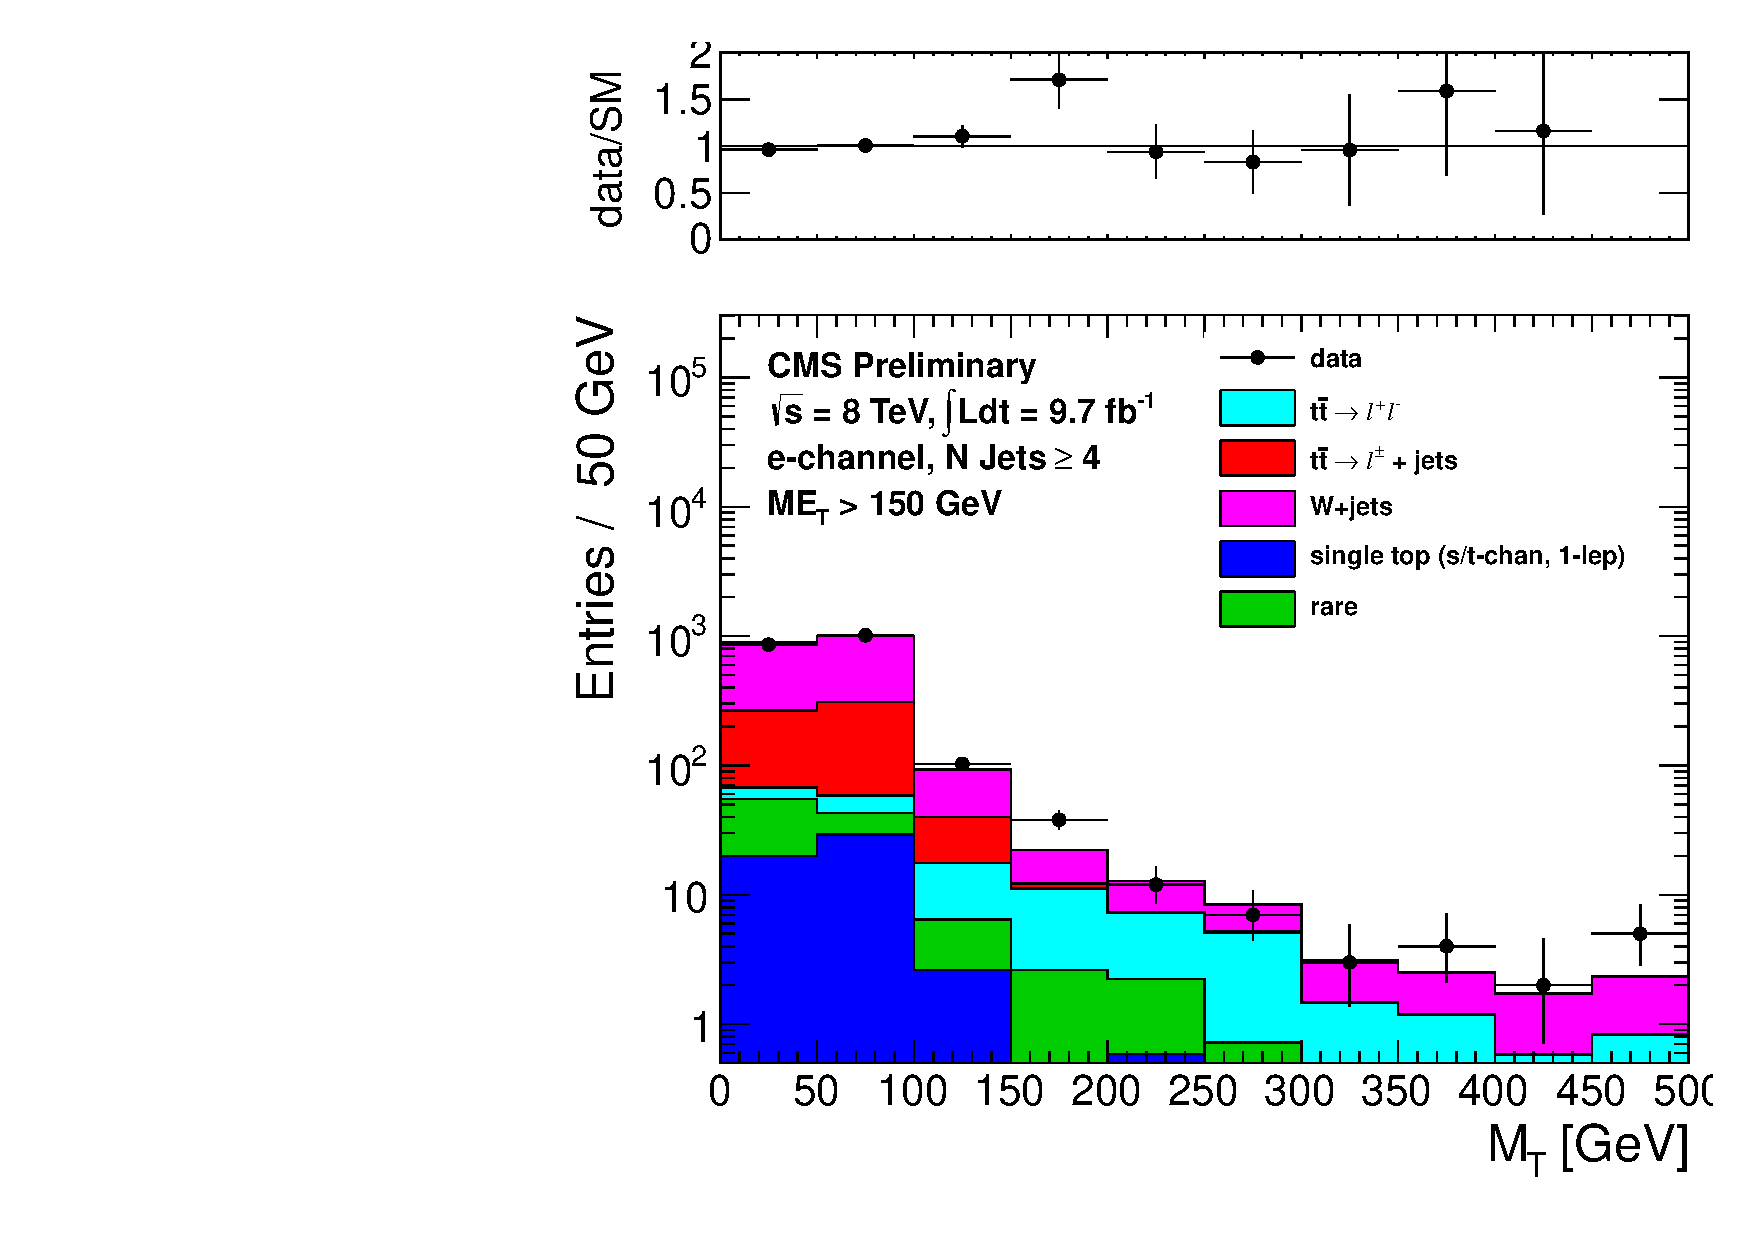
\includegraphics[width=0.5\linewidth]{plots/CR1plots/mt_met150_leadele_nj4.pdf}
        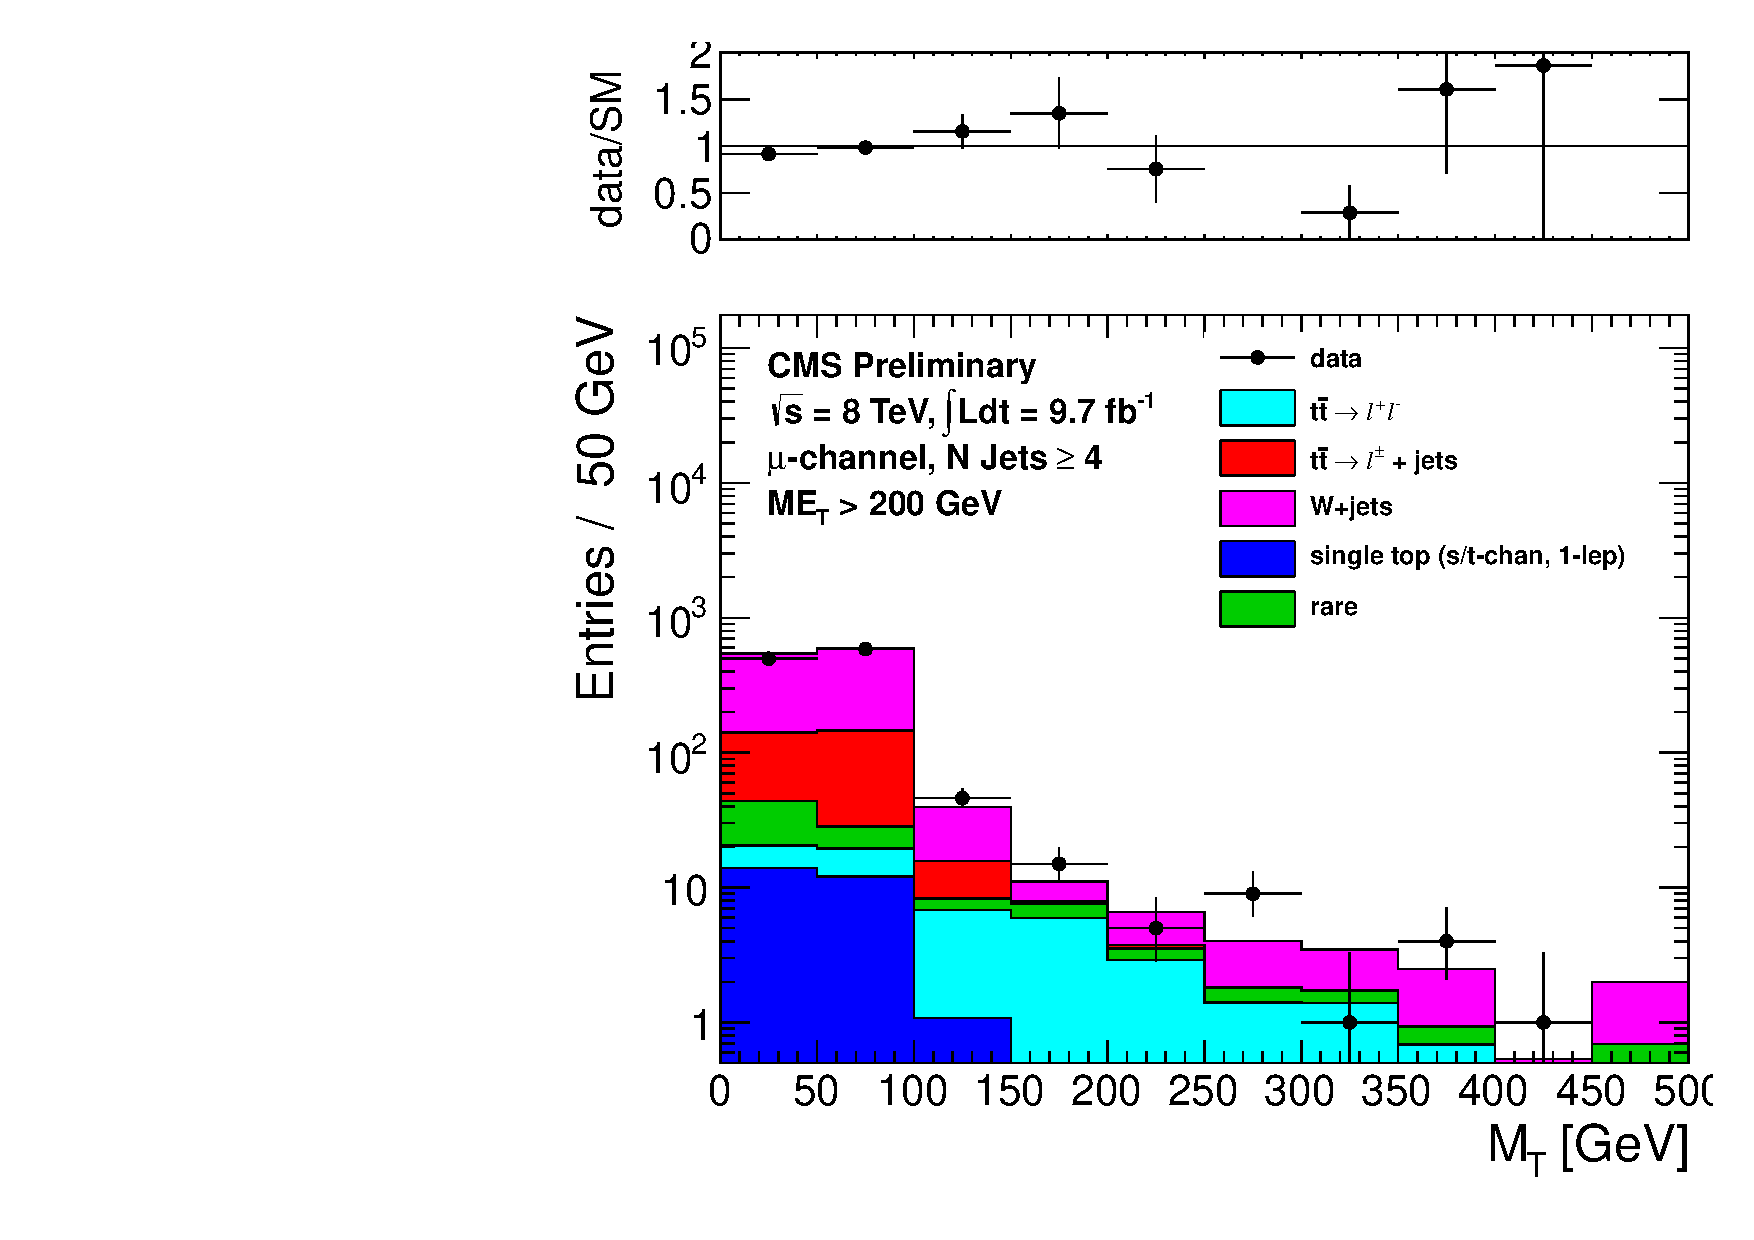
\includegraphics[width=0.5\linewidth]{plots/CR1plots/mt_met200_leadmuo_nj4.pdf}%
        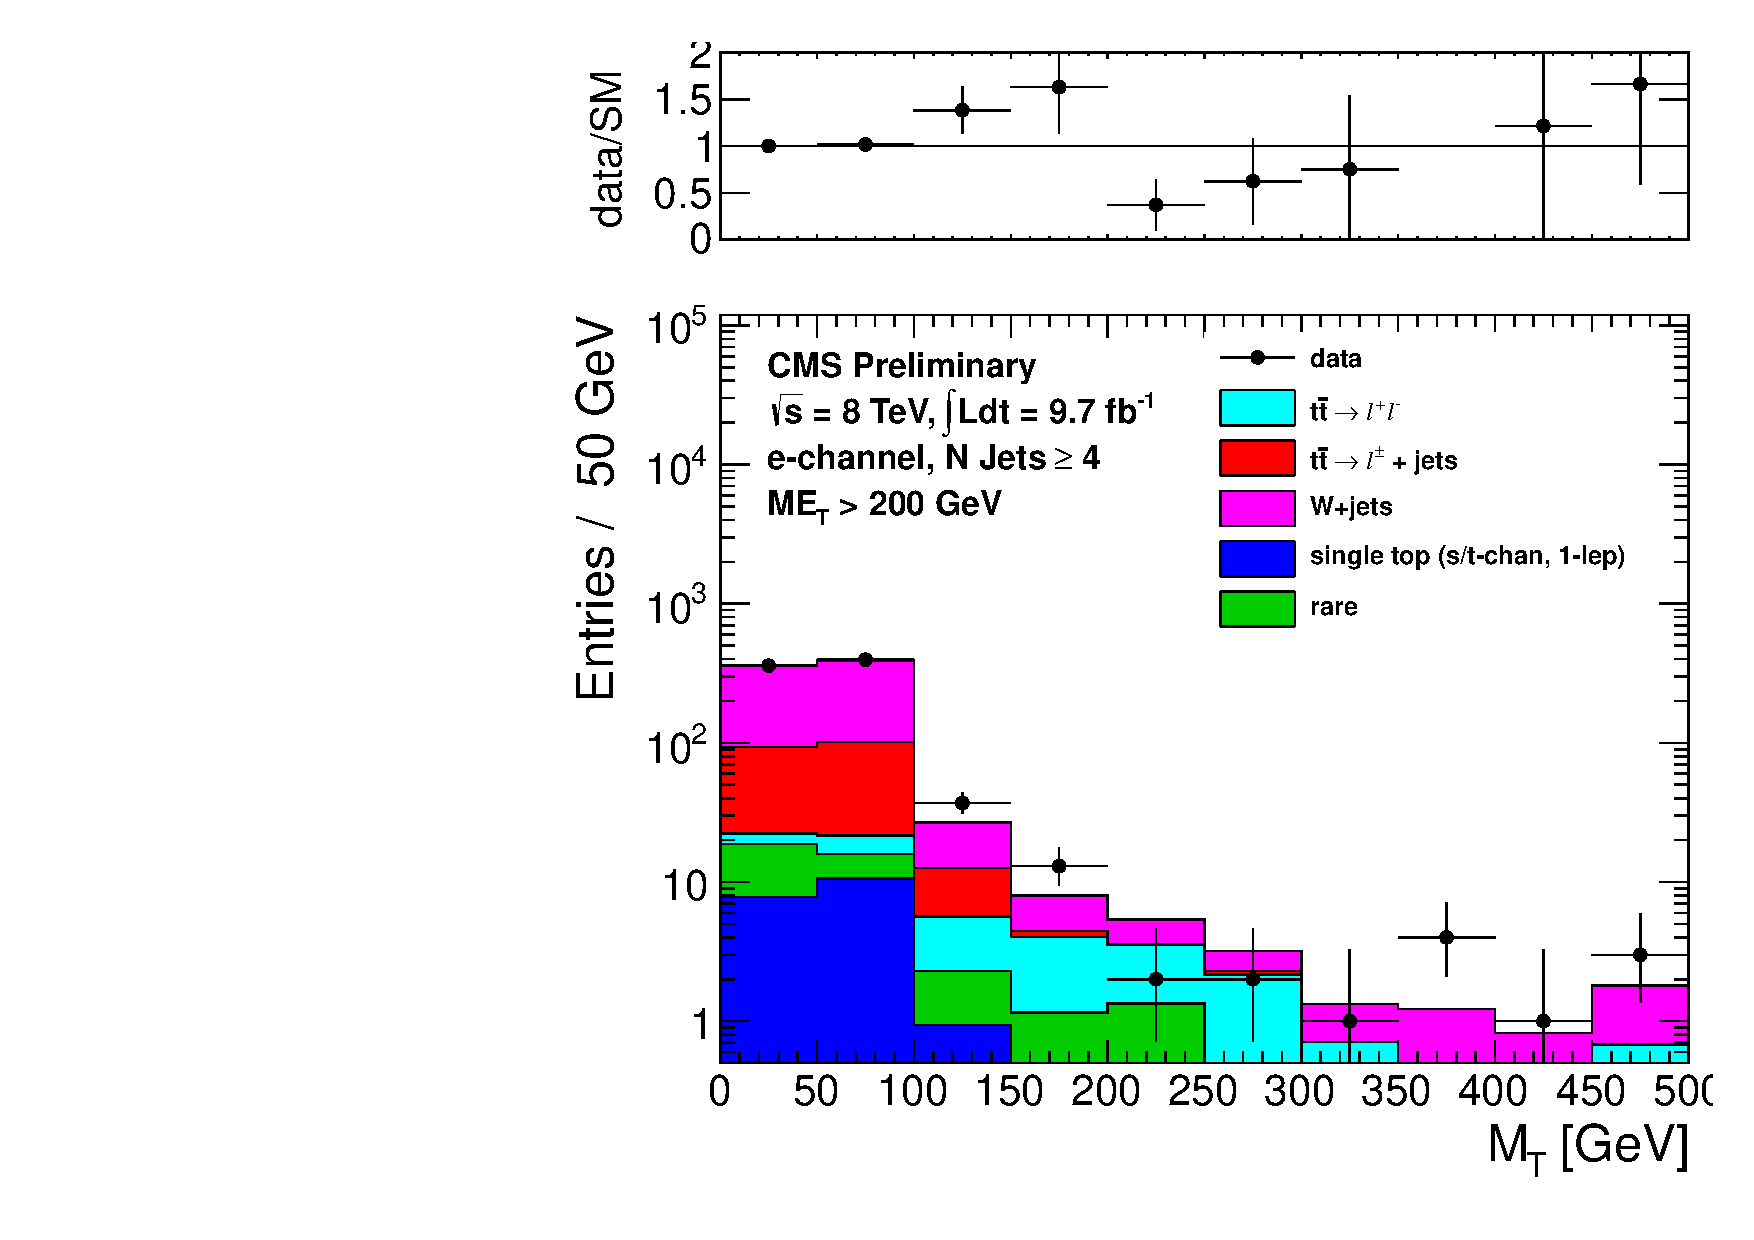
\includegraphics[width=0.5\linewidth]{plots/CR1plots/mt_met200_leadele_nj4.pdf}
        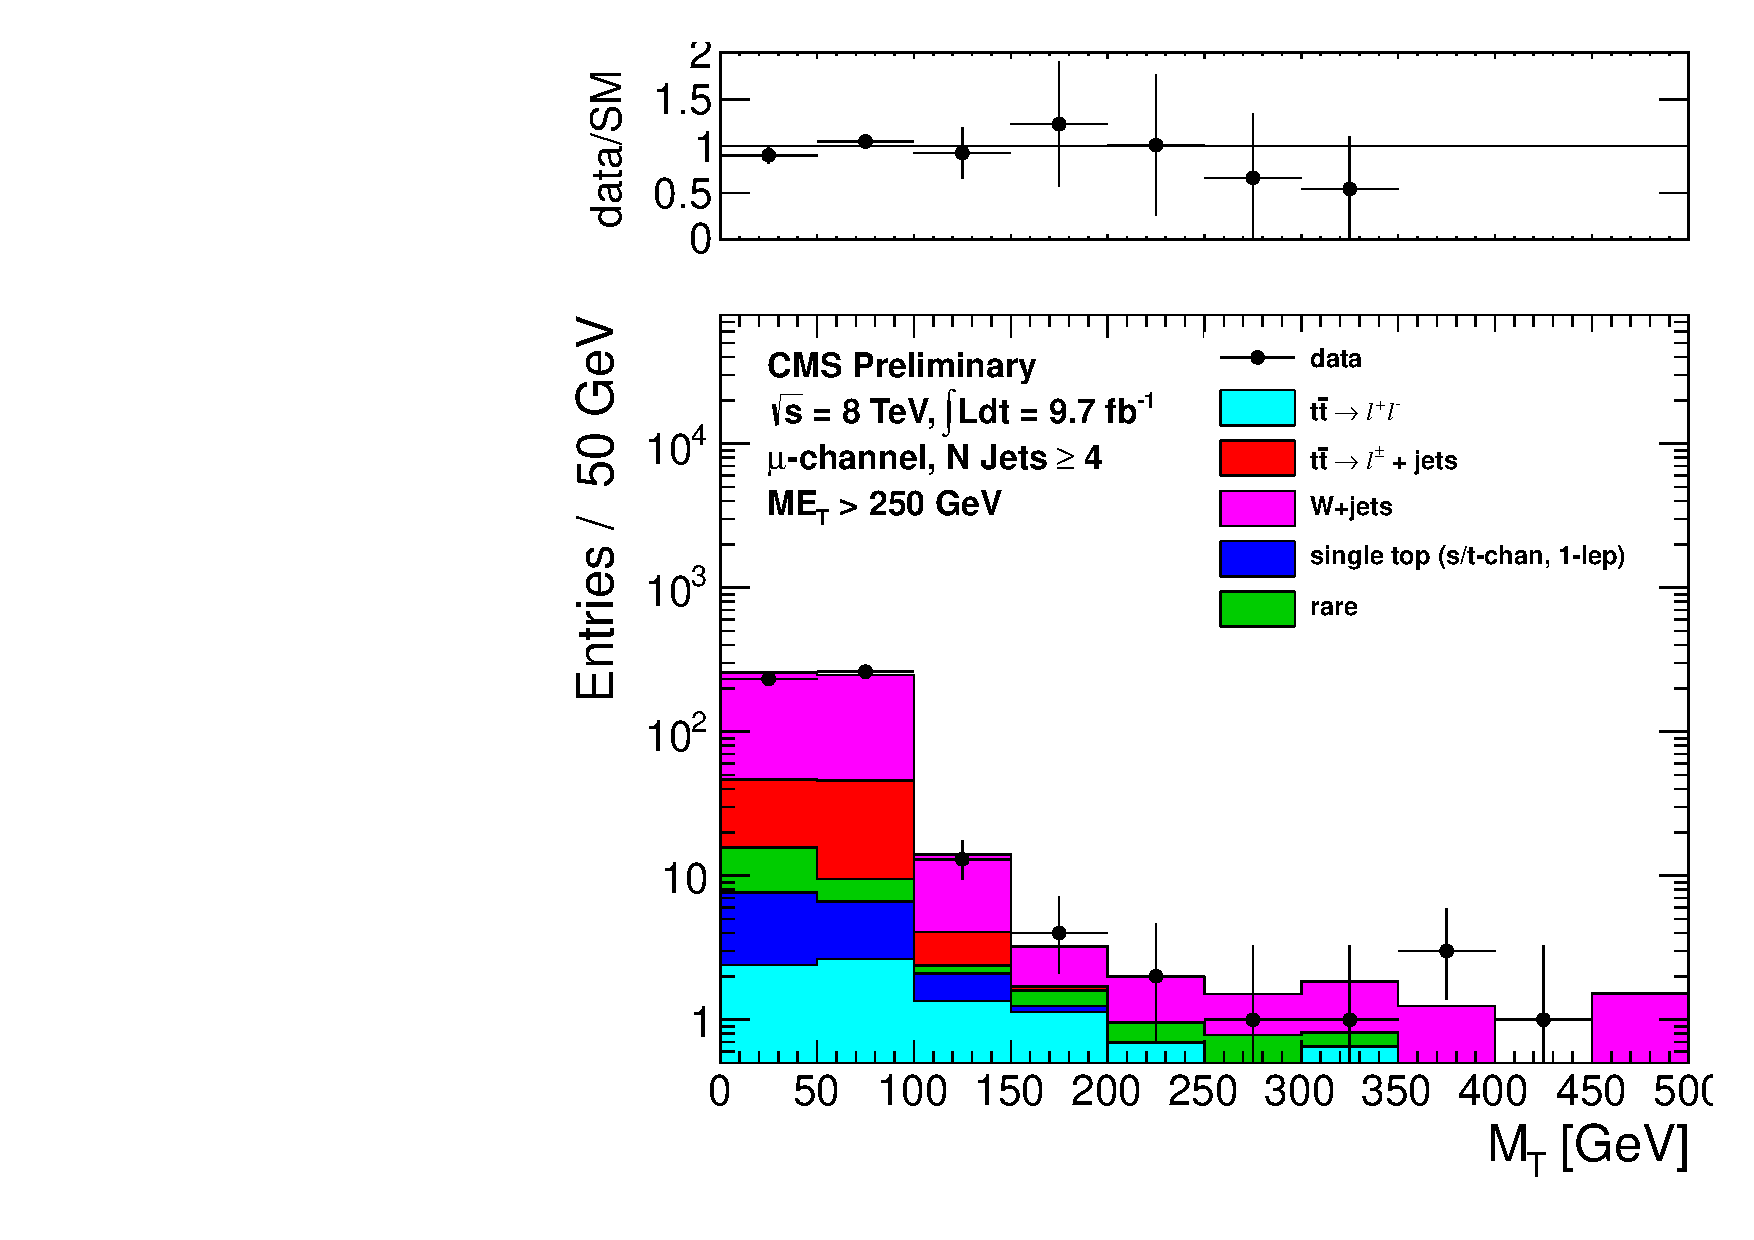
\includegraphics[width=0.5\linewidth]{plots/CR1plots/mt_met250_leadmuo_nj4.pdf}%
        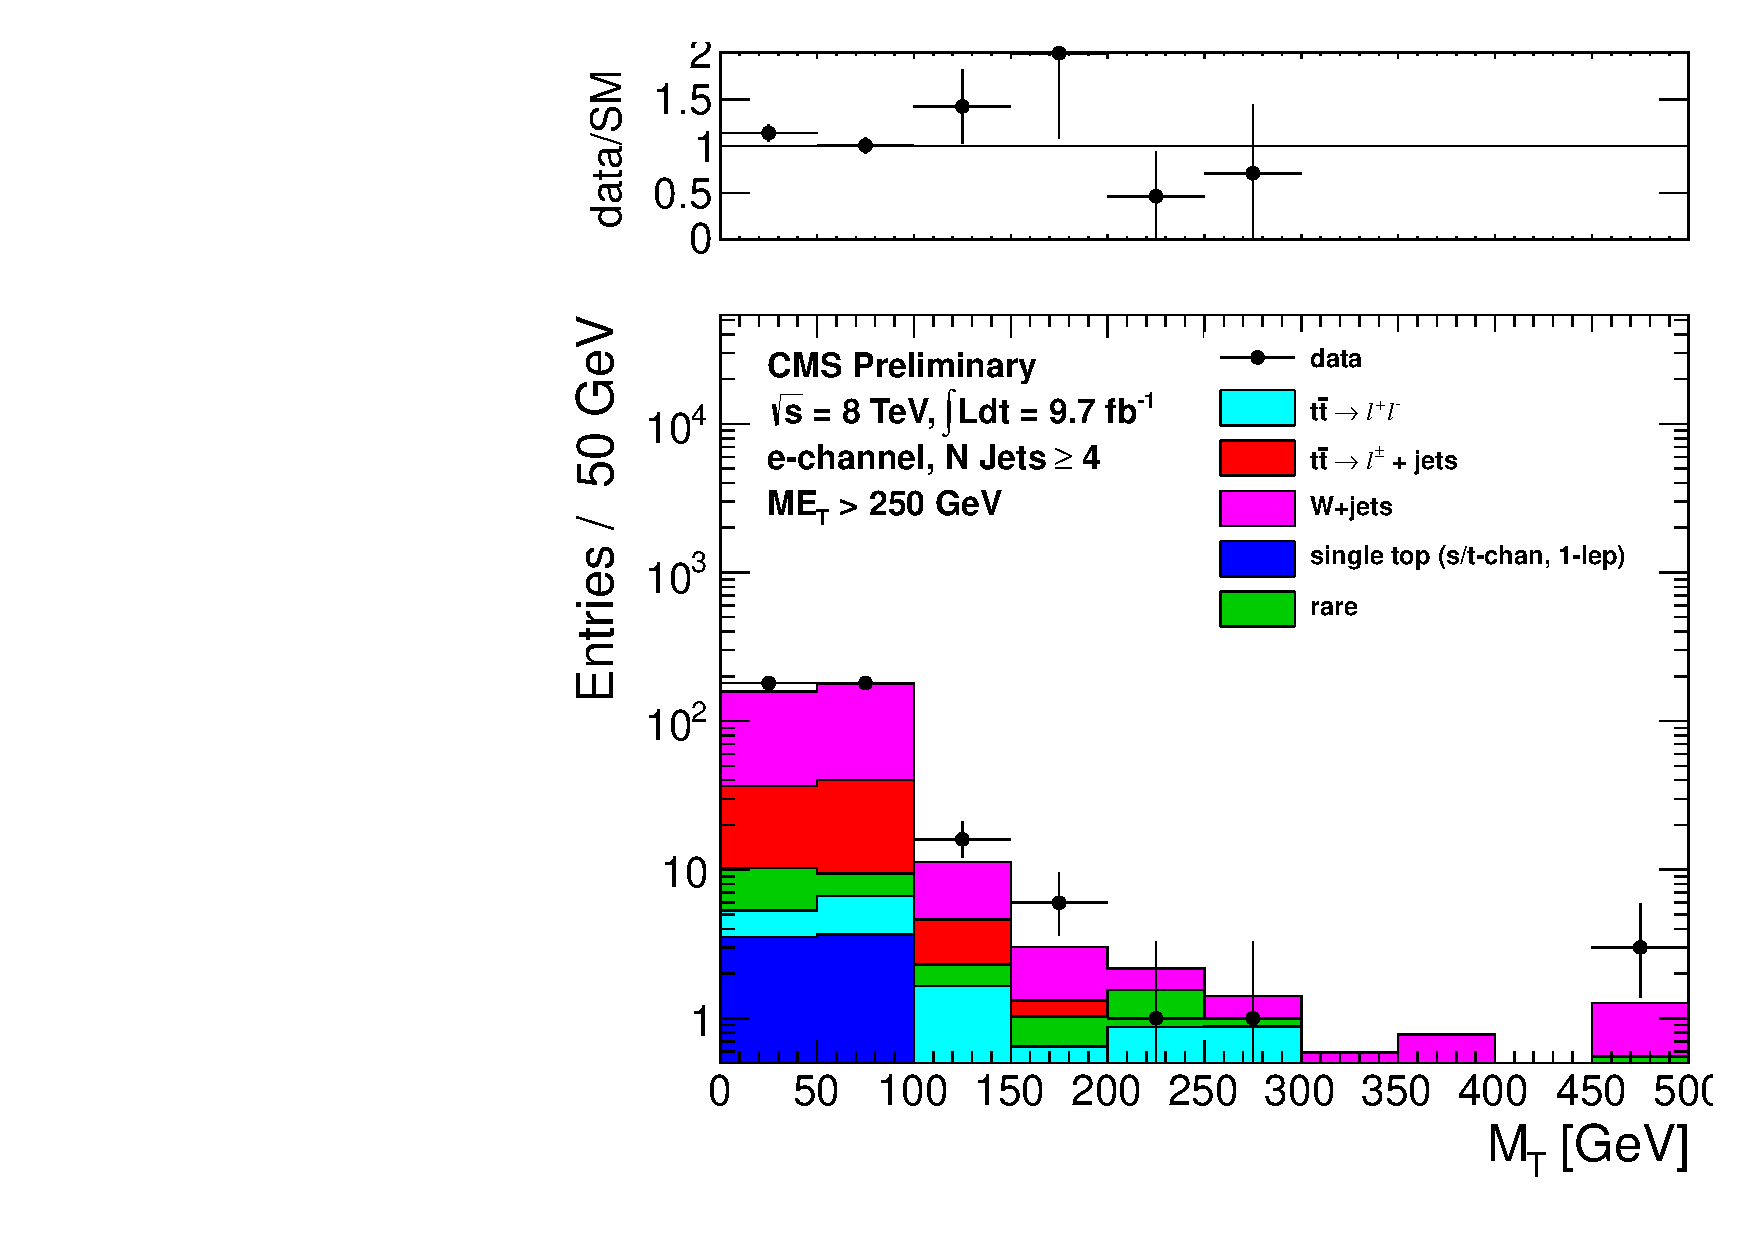
\includegraphics[width=0.5\linewidth]{plots/CR1plots/mt_met250_leadele_nj4.pdf}
    \caption{
      Comparison of the \mt\ distribution in data vs. MC for events
      with a leading muon (left) and leading electron (right)
      satisfying the requirements of CR1. The \met\ requirements used are
      150 GeV (top), 200 GeV (middle) and 250 GeV (bottom).
\label{fig:cr1mtrest} 
}  
      \end{center}
\end{figure}

\begin{figure}[hbt]
  \begin{center}
        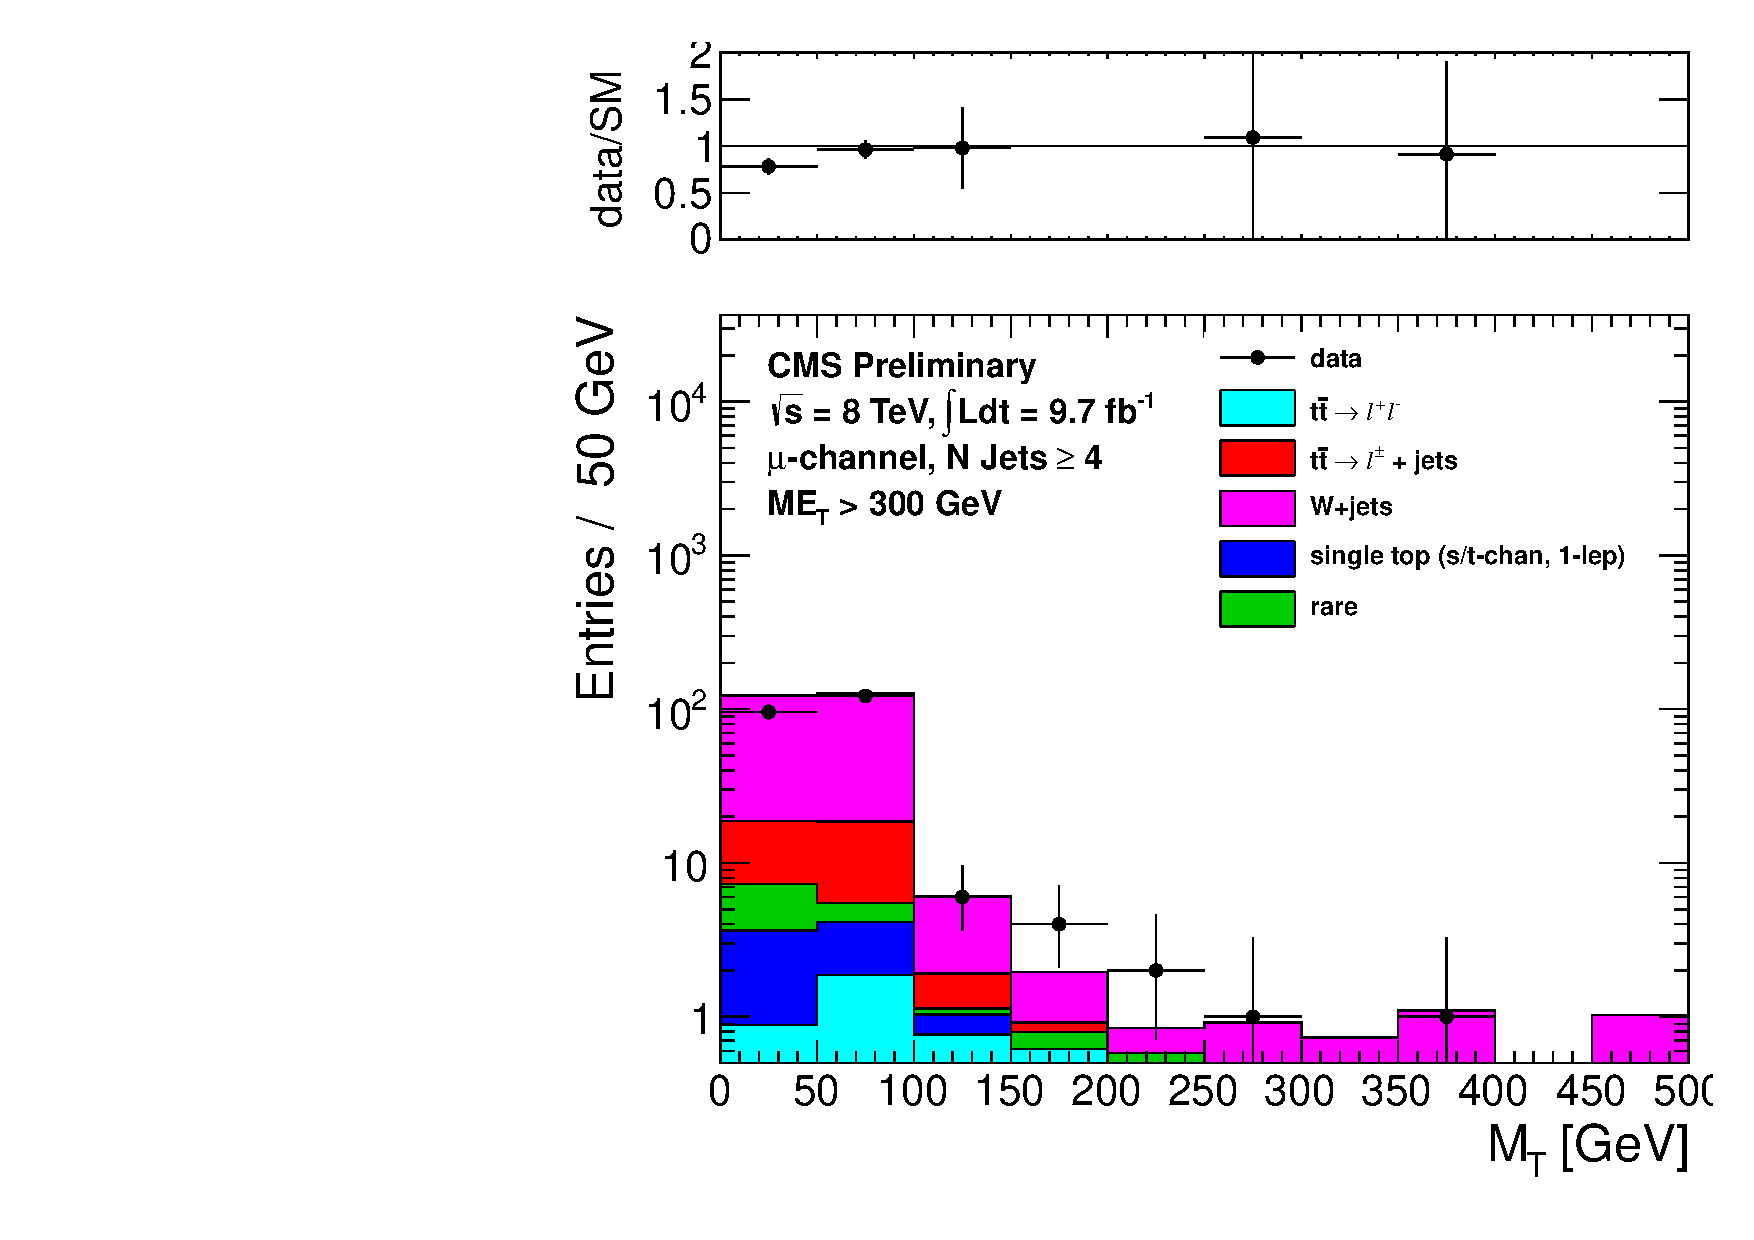
\includegraphics[width=0.5\linewidth]{plots/CR1plots/mt_met300_leadmuo_nj4.pdf}%
        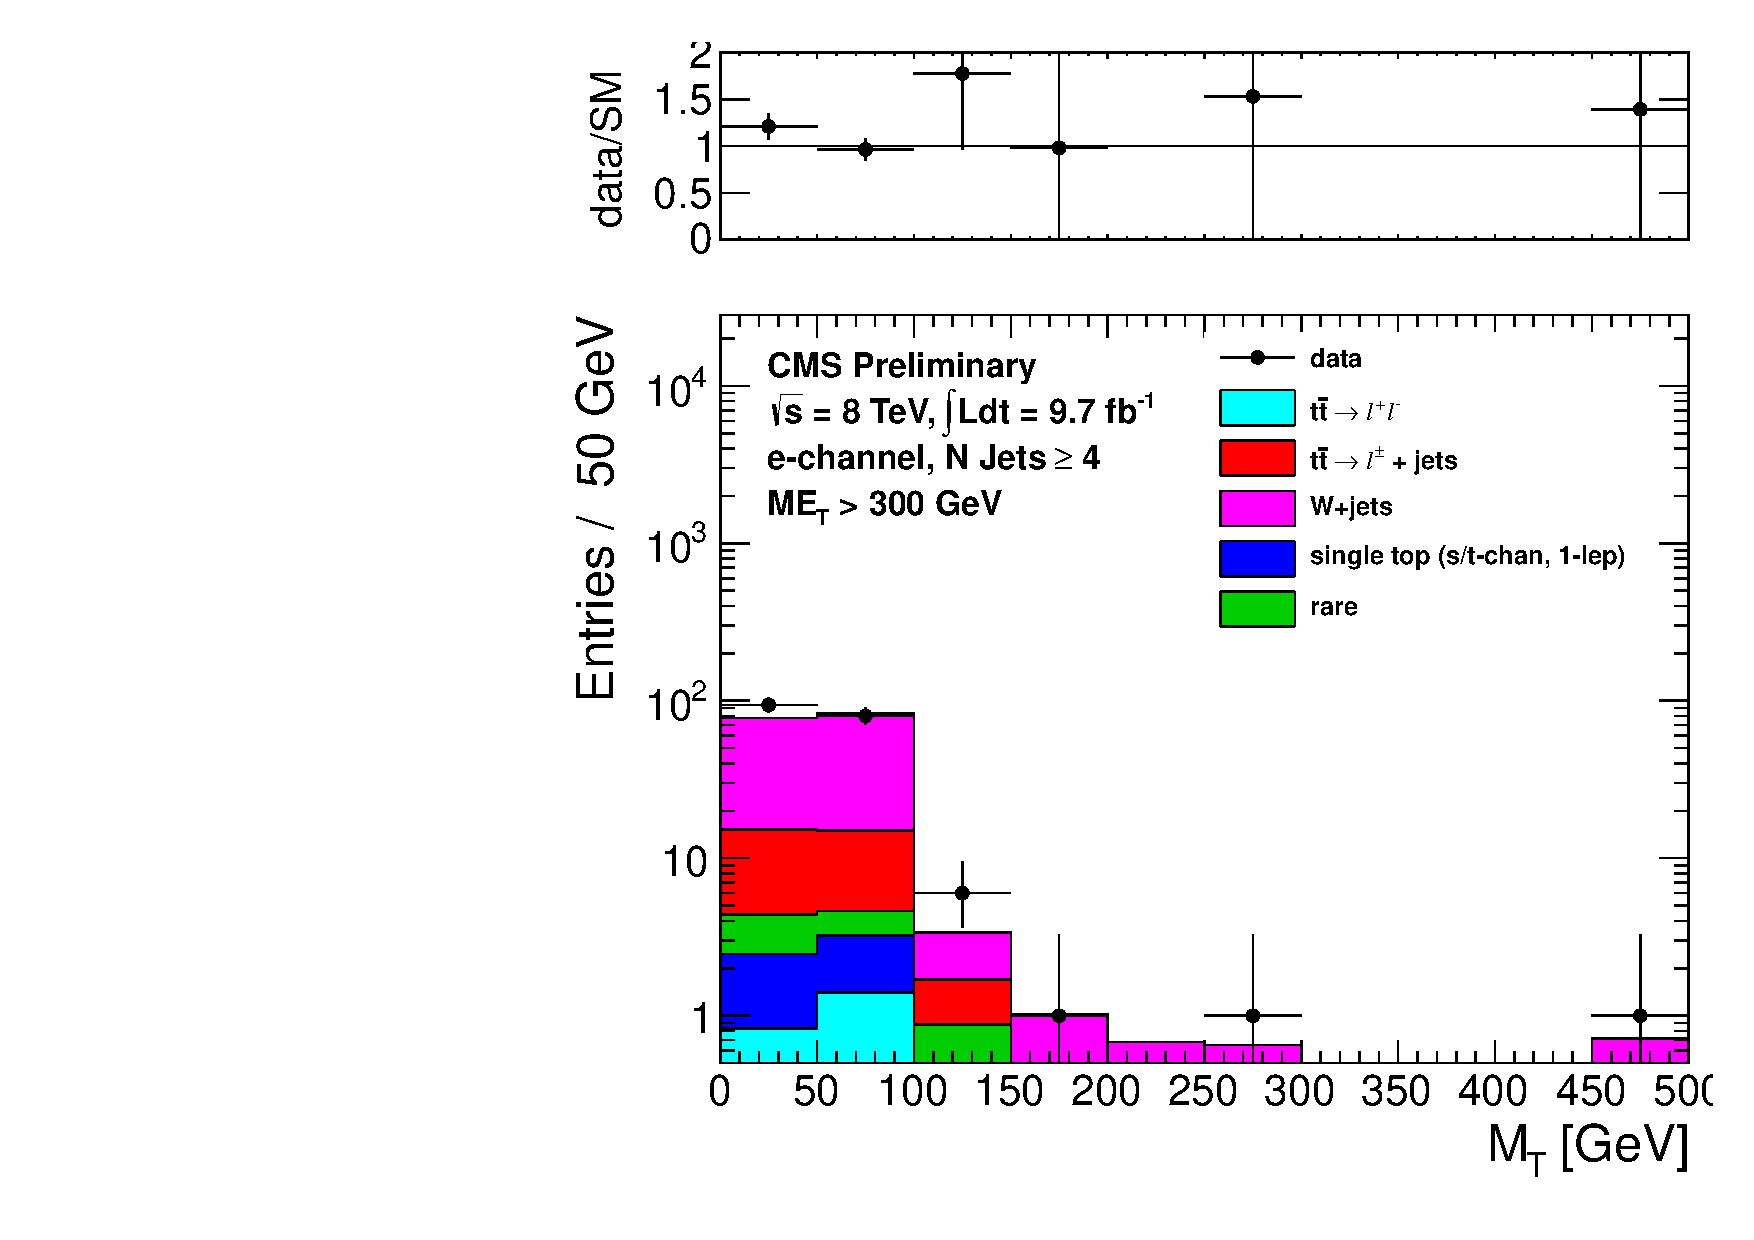
\includegraphics[width=0.5\linewidth]{plots/CR1plots/mt_met300_leadele_nj4.pdf}
        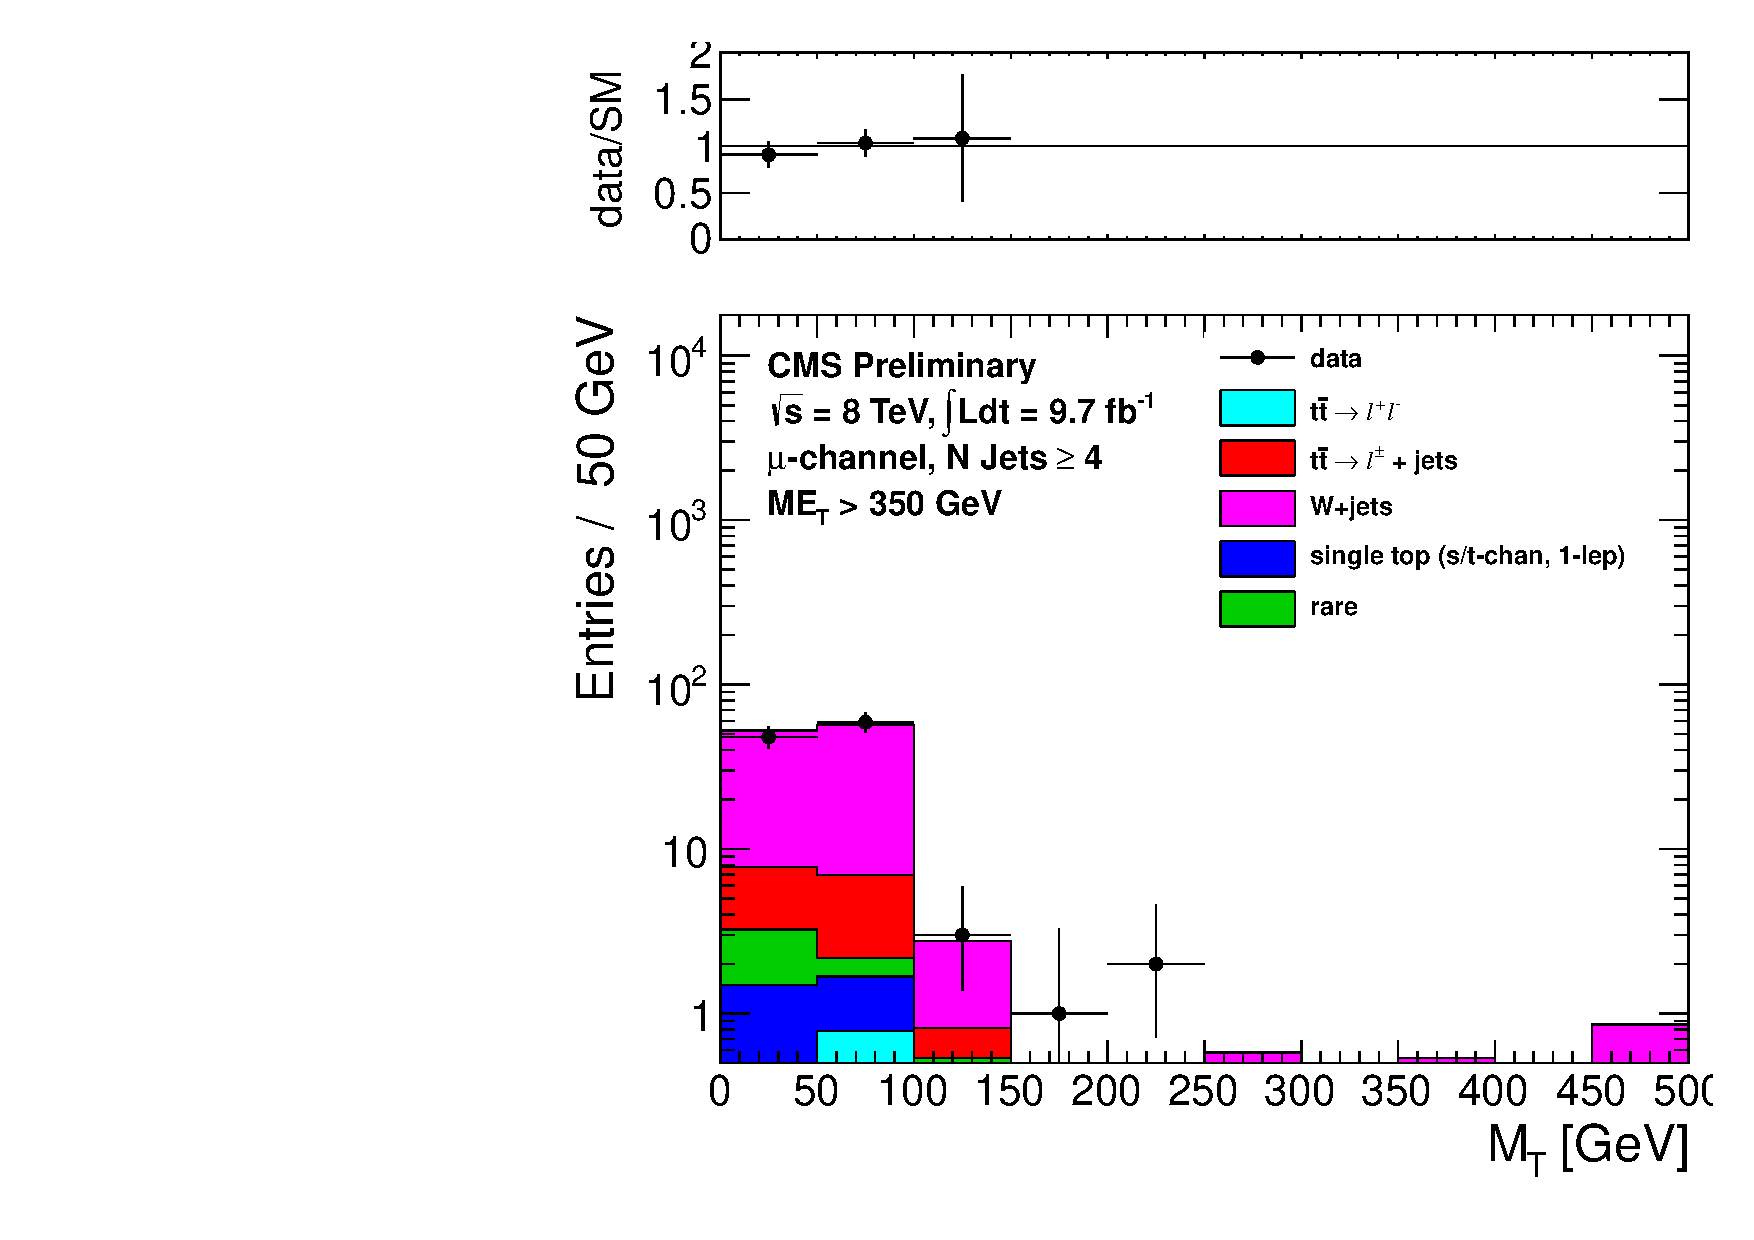
\includegraphics[width=0.5\linewidth]{plots/CR1plots/mt_met350_leadmuo_nj4.pdf}%
        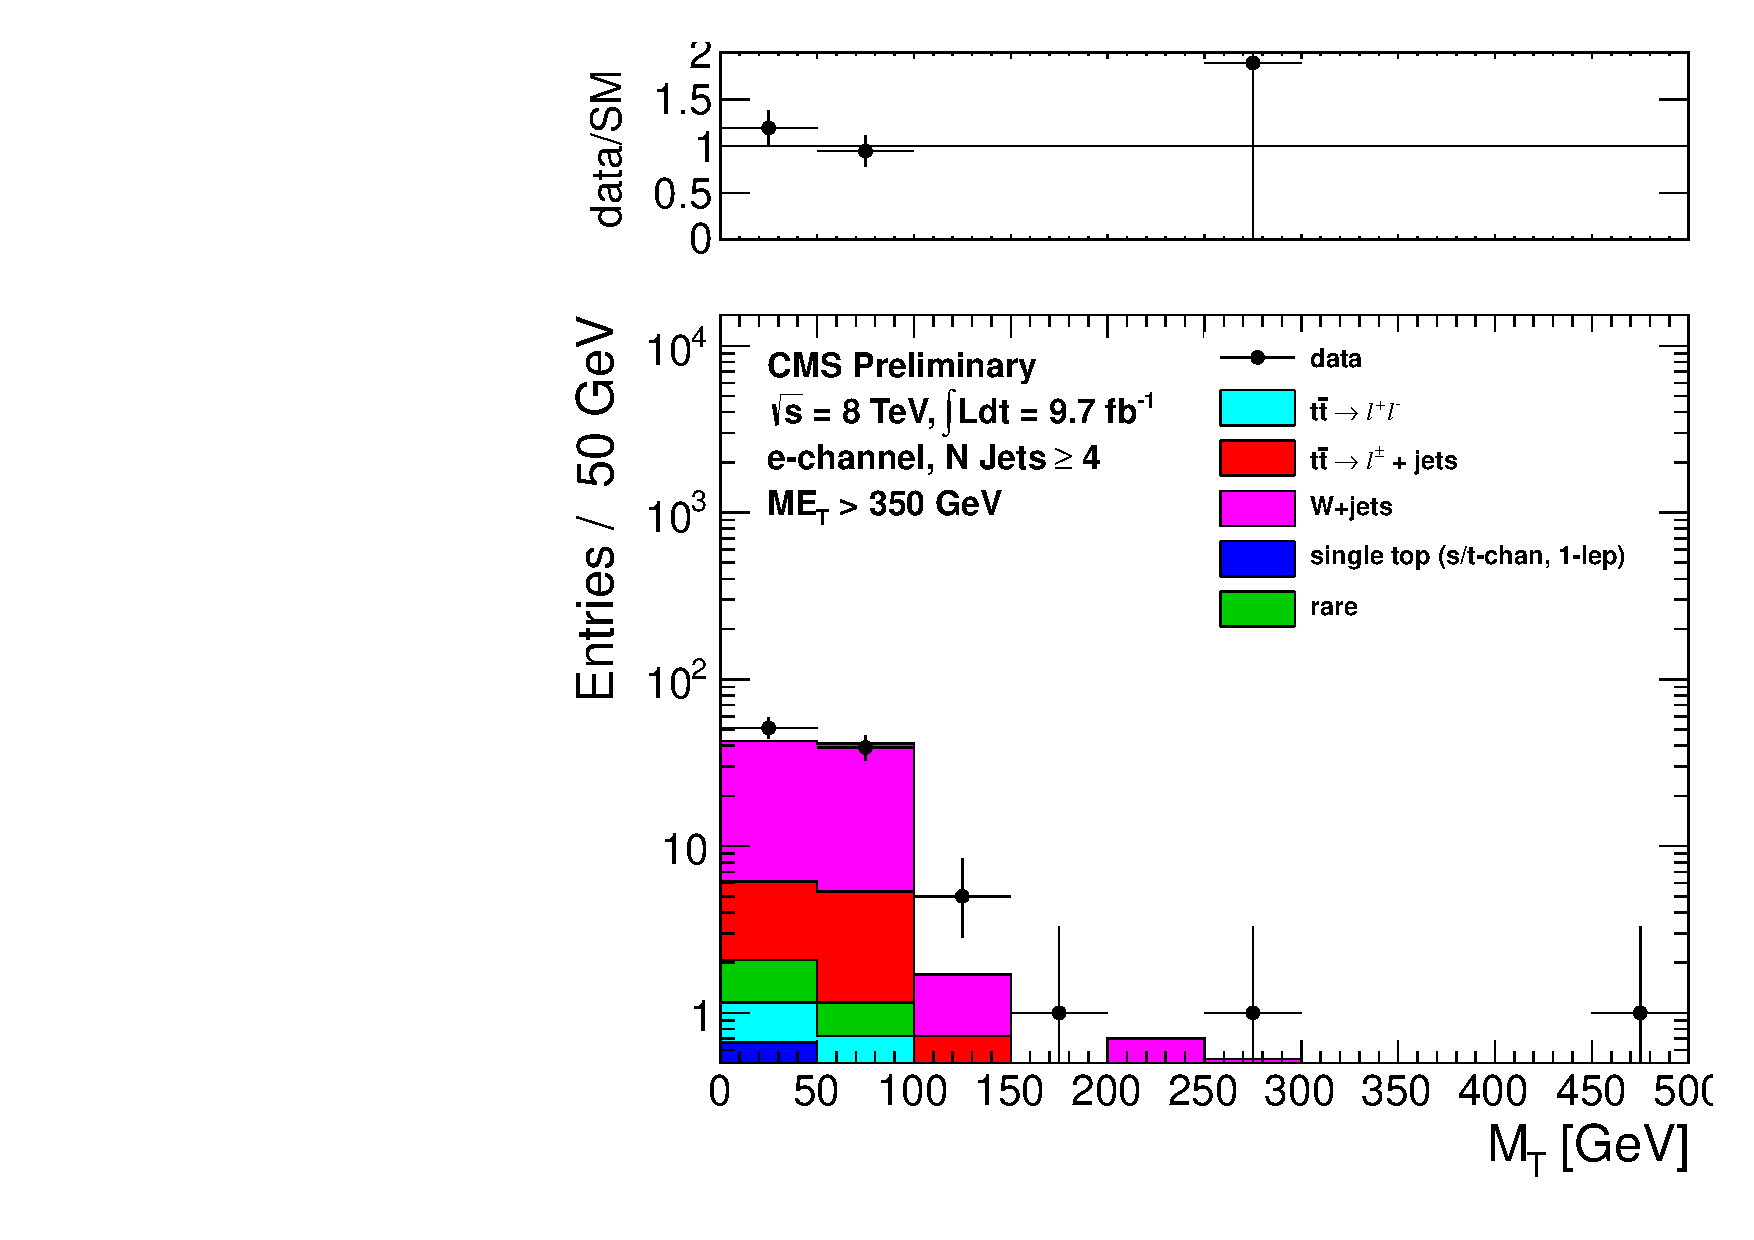
\includegraphics[width=0.5\linewidth]{plots/CR1plots/mt_met350_leadele_nj4.pdf}
        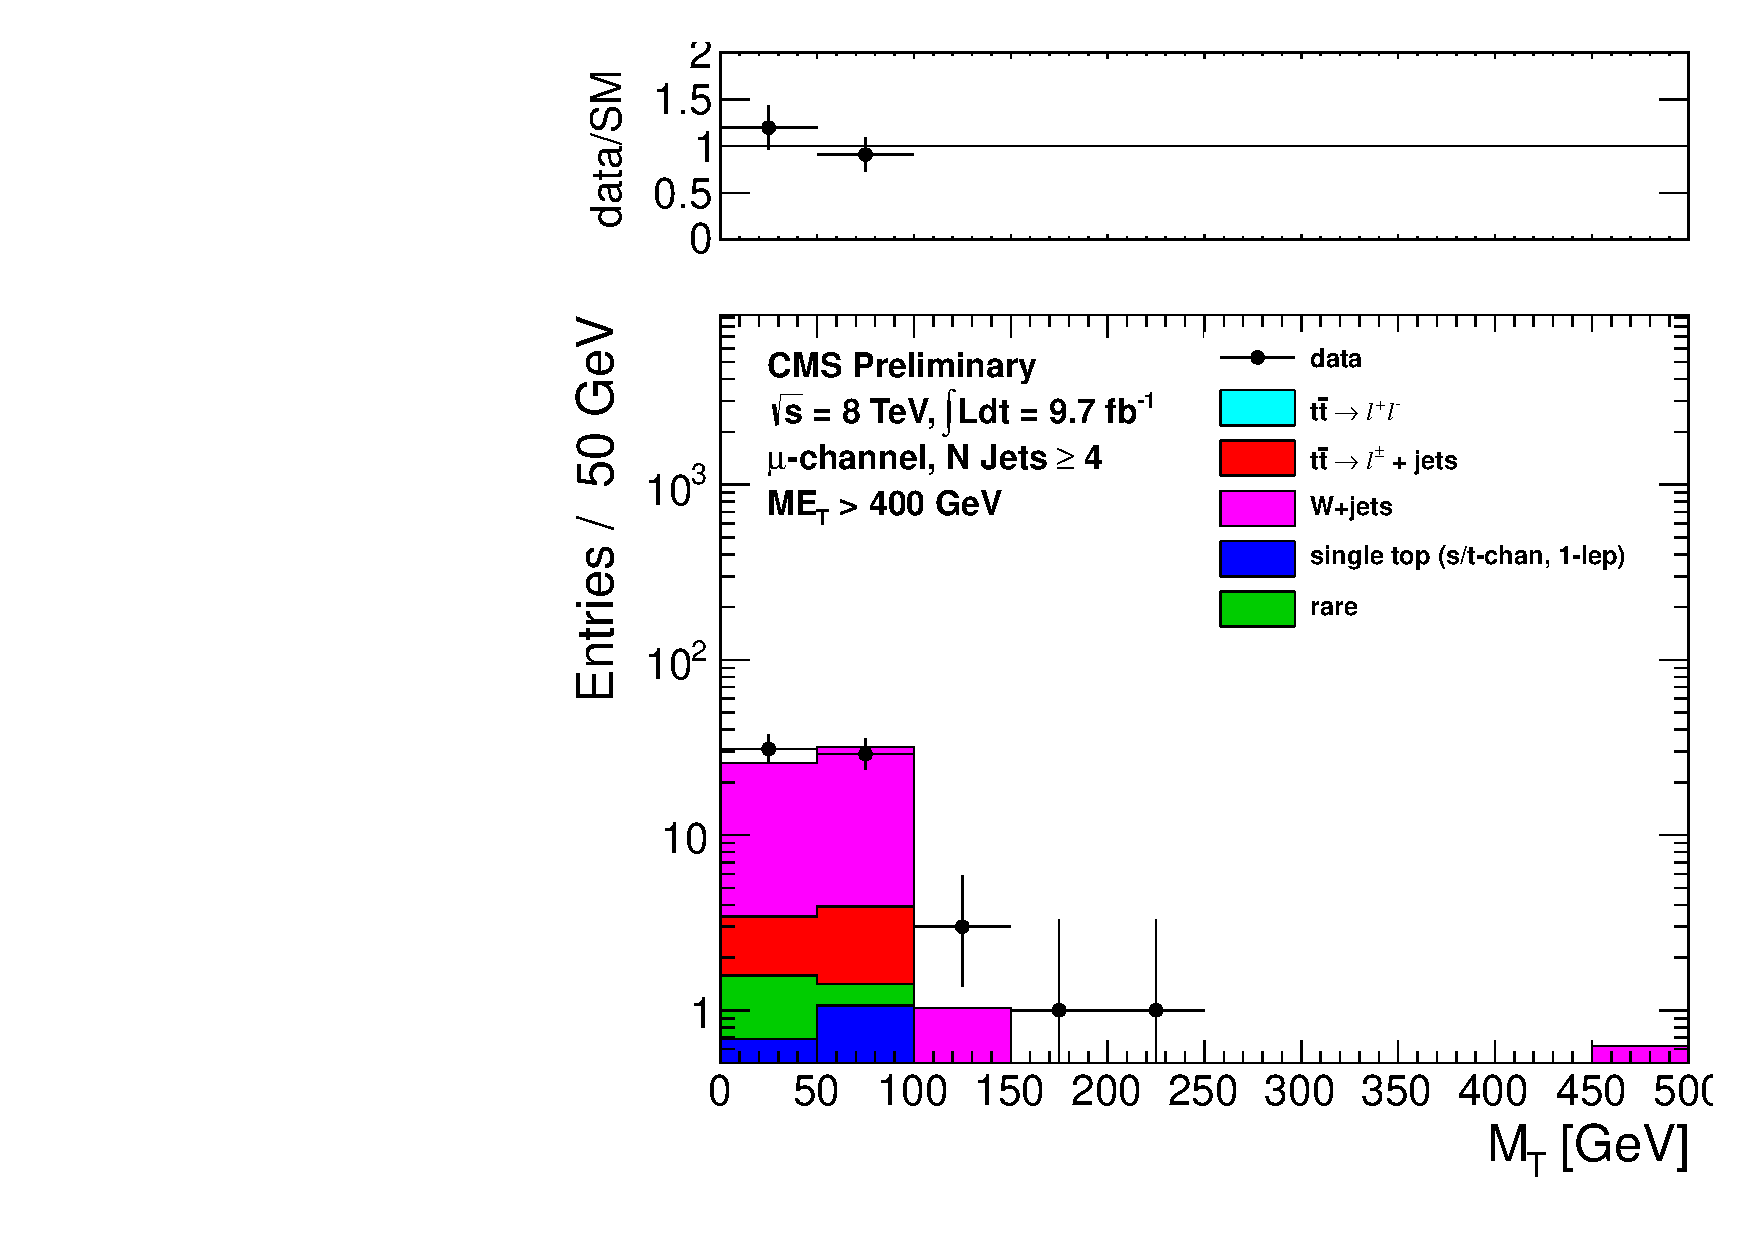
\includegraphics[width=0.5\linewidth]{plots/CR1plots/mt_met400_leadmuo_nj4.pdf}%
        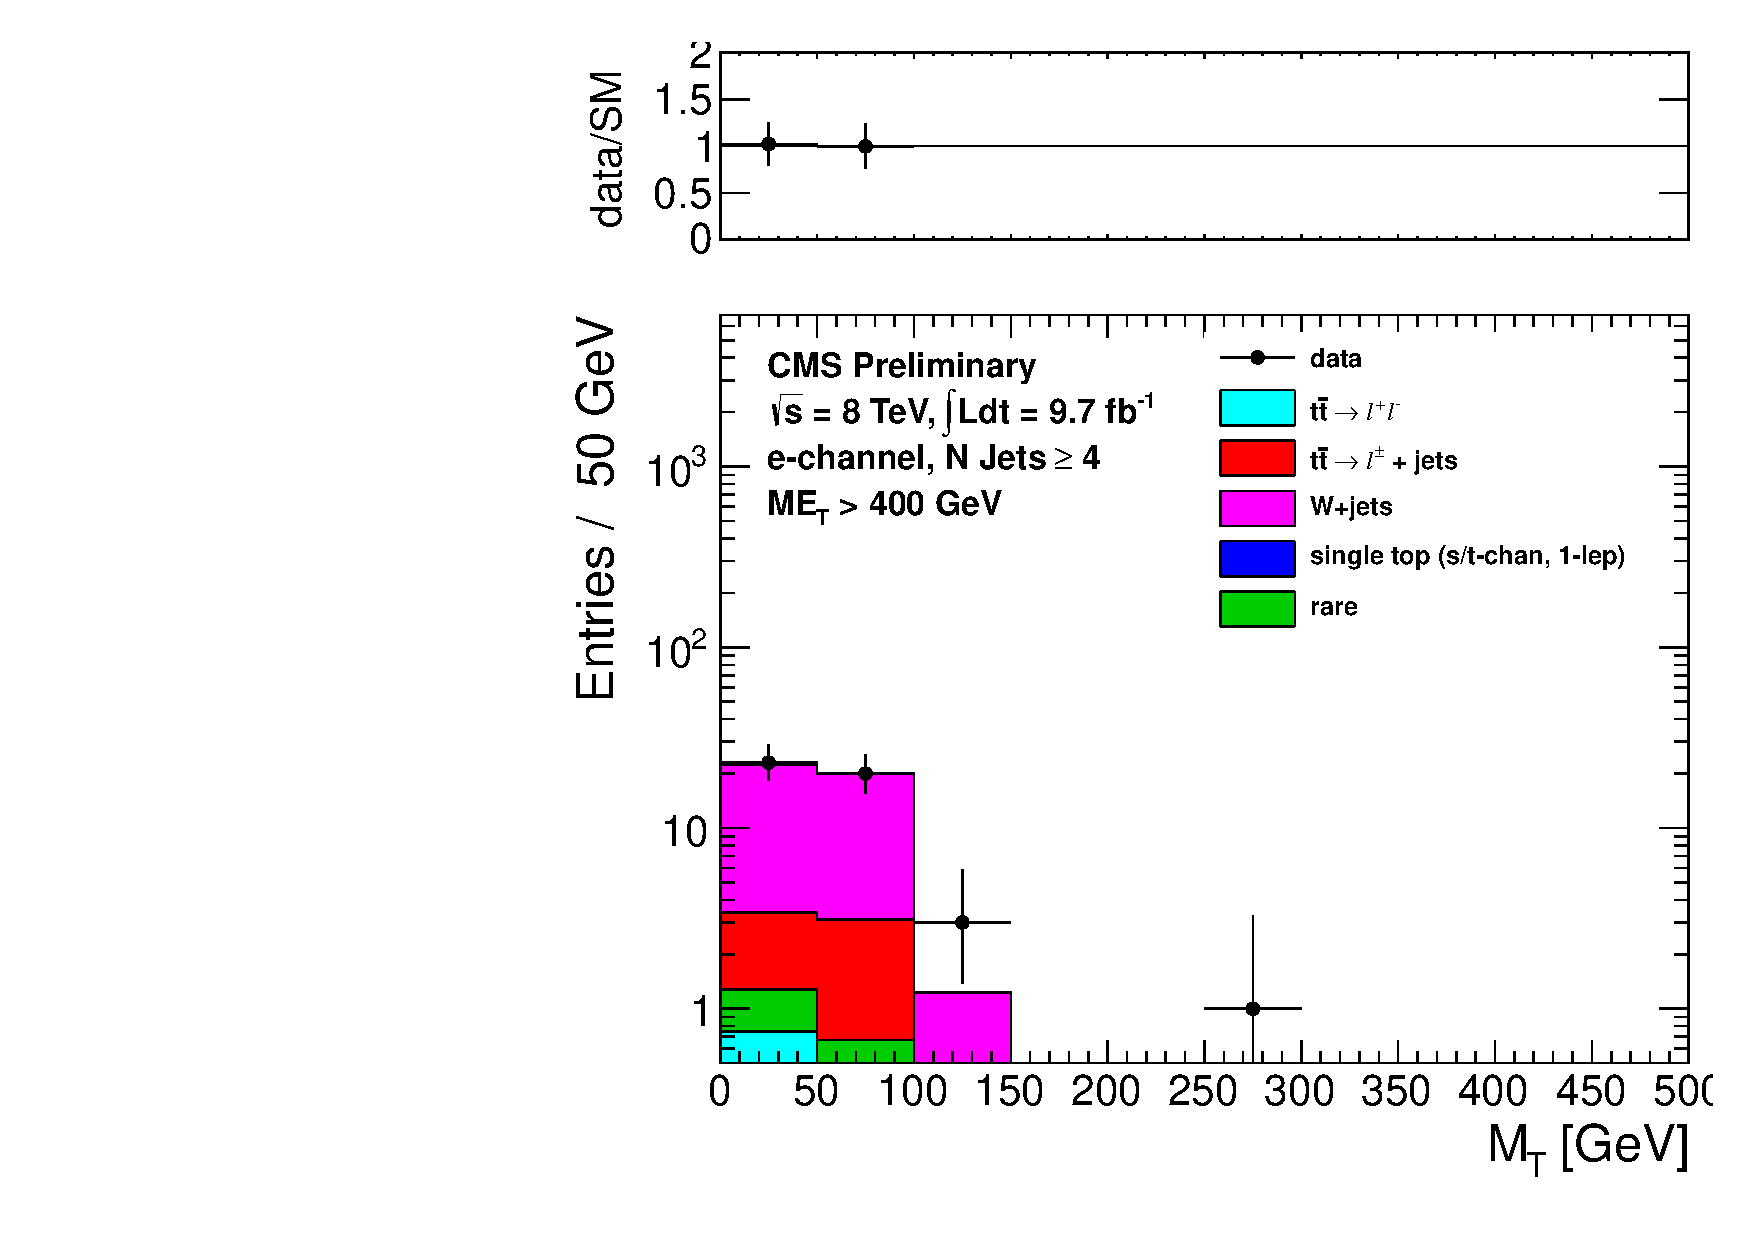
\includegraphics[width=0.5\linewidth]{plots/CR1plots/mt_met400_leadele_nj4.pdf}
    \caption{
      Comparison of the \mt\ distribution in data vs. MC for events
      with a leading muon (left) and leading electron (right)
      satisfying the requirements of CR1. The \met\ requirements used are
      300 GeV (top), 350 GeV (middle) and 400 GeV (bottom).
\label{fig:cr1mtrest2} 
}  
      \end{center}
\end{figure}


\clearpage
